% !TeX spellcheck = en_US


\chapter{Fast Spectral Method for Linear Gas Flows}
\label{chap:linearized}
\index{linearized Boltzmann equation}

The FSM is applied to solve the linearized Boltzmann equation. First, two canonical problems in rarefied gas dynamics, the Poiseuille flow and thermal transpiration, are simulated and compared to solutions of the numerical kernel method. Because of the ``over-concentration'' in velocity distribution function~\cite{Takata2011}, numerical simulation of highly rarefied gas flows is a difficult task; for a long time the accurate numerical results have been limited to HS molecules when $\text{Kn}\lesssim20$~\cite{Ohwada_sone_1989,Doi2010}. Here the LBE is solved accurately and efficiently by FSM, up to $\text{Kn}\sim10^6$. 
Then, the LBE with collision kernels directly calculated from the Lennard-Jones potential is solved. Third, the role of intermolecular potential on rarefied gas flows is studied. 

%Finally, the rarefied gas flow through the porous media represented by Sierpinski carpets is simulated.  


% Recently, some progresses have been achieved both analytically and numerically, where the results are obtained at large Knudsen numbers~\cite{Takata2011,Funagane2012,Doi2012,Doi2012b}. 


\section{Linearization}\label{linearization_FSM}
\index{Linearization}

The linearized Boltzmann collision operator~\eqref{BCO_lin_chapter1} cannot be solved by FSM, because in general the perturbation function $\phi(-L_v)\neq\phi(L_v)$. However, the product of the equilibrium distribution function and $\phi$ vanishes at large molecular speed. Therefore, the Boltzmann equation is linearized by expressing the VDF as (the normalization in Chapter~\ref{Normalization_FSM} is used):
\begin{equation}\label{Chapter_lin_VDF}
f(t,\bm{x},\bm{v})=f_{eq}(\bm{v})+\beta{}h(t,\bm{x},\bm{v})
\end{equation}
with the equilibrium distribution function
\begin{equation}\label{equilibrium_Maxwellian_lin}
f_{eq}(\bm{v})=\pi^{-3/2}\exp(-v^{2}),
\end{equation}
where $\beta$ is a small constant related to the dimensionless strength of perturbation (e.g. in the linear Couette flow $\beta$ can be the wall velocity divided by the most probable speed), and $\beta{}h$ is the distribution function for small perturbation, that is, $|\beta{}h/f_{eq}|\ll1$. The Boltzmann equation~\eqref{Boltzmann} is linearized to
\begin{equation}\label{Chapter1_Boltzmann_lin}
\frac{\partial {h}}{\partial t}+\bm{v}\cdot\frac{\partial{h}}{\partial
	\bm{x}}
-2\bm{a}\cdot\bm{v}f_{eq}=\mathcal{L}(h)\equiv{}\mathcal{L}^+-\nu_{eq}(\bm{v}){h},
\end{equation}
where 
\begin{equation}\label{linearized1}
\mathcal{L}^+(h)=\iint B(\theta,v_r)  [f_{eq}(\bm{v}')h({\bm{v}}'_{\ast})+f_{eq}(\bm{v}'_\ast)h({\bm{v}}')-f_{eq}(\bm{v})h({\bm{v}}_\ast)]d\Omega d{\bm{v}}_\ast
\end{equation}
can be viewed as a gain term of the linearized Boltzmann collision operator, while $\nu_{eq}(\bm{v}){h}$ is the loss term, with the equilibrium collision frequency (or loss rate) being
\begin{equation}\label{linearized2}
\nu_{eq}(\bm{v})=\iint{}B(\theta,{v}_r)f_{eq}(\bm{v}_{\ast}) d\Omega{d\bm{v}_\ast}.
\end{equation} 









%
%In the present paper, we \lei{mainly} consider the inverse power-law potentials, where the collision kernels are modeled as~\cite{Lei2013,lei_Jfm}
%\begin{equation}\label{collision_kernel}
%B(|{\bm{u}}|,\theta)=\frac{|{\bm{u}}|^{2(1-\omega)}}{K}	{\sin^{\frac{1}{2}-\omega}\left(\frac{\theta}{2}\right)\cos^{\frac{1}{2}-\omega}\left(\frac{\theta}{2}\right)},
%\end{equation}
%with $\omega$ being the viscosity index (i.e. the shear viscosity $\mu$ of the gas is proportional to $T^\omega$) and $K$ some normalization constants~\cite{lei_Jfm}. HS and Maxwell molecules have $\omega=0.5$ and 1, respectively. \lei{We will also consider the Lennard-Jones potentials (the detailed implementation of which by the fast spectral method can be found in Ref.~\cite{Wu:2015yu}) to demonstrate that the GSIS works for the LBE with general intermolecular potentials}.







The macroscopic quantities deviated from their corresponding values in equilibrium state, such as the number density $\varrho$, bulk velocity $\bm{u}$, temperature $T$, stress tensor $\sigma_{ij}$ and heat flux $\bm{q}$ can be calculated as
\begin{equation}\label{MP}
[\varrho,\bm{u},T,\sigma_{ij},\bm{q}]=
\int\left[1,\bm{v},\frac{2}{3}\left(v^2-\frac{3}{2}\right),2v_{\langle i}v_{j\rangle},\left({v^2}-\frac{5}{2}\right)\right]{h}d\bm{v},
\end{equation}
which, on top of the normalization~\eqref{normalization}, are further normalized by the dimensionless constant $\beta$.


The equilibrium collision frequency can be calculated analytically, or approximated by the algorithm 2 in Appendix~\ref{appen_FSM}, if $\hat{f}$ is replaced by the spectrum of  equilibrium distribution function $\hat{f}_{eq}$. This term only needs to be calculated once, since each spatial cell uses the same equilibrium collision frequency. For the gain term $\mathcal{L}^+$, if Eq.~\eqref{kernel_mode2} is approximated by Gauss-Legendre quadrature, its $j$-th Fourier mode is 
\begin{equation}\label{detailed_linear}
\begin{aligned}[b]
\widehat{\mathcal{L}}^+_{\bm{j}}\approx &\frac{4}{\text{Kn}'}\sum_{p,q=1}^{M} \sum_{\bm{l}+\bm{m}=\bm{j}}\omega_p\omega_q\sin\theta_p[\hat{f}_{eq}(\bm{l}){\phi_{\alpha+\gamma}(\xi_{\bm{l}},\theta_p,\varphi_q)}]\cdot[\hat{h}_{\bm{m}}{\psi_{\gamma}(\xi_{\bm{m}},\theta_p,\varphi_q)}]\\
+&\frac{4}{\text{Kn}'}\sum_{p,q=1}^{M} \sum_{\bm{l}+\bm{m}=\bm{j}}\omega_p\omega_q\sin\theta_p[\hat{h}_{\bm{l}}{\phi_{\alpha+\gamma}(\xi_{\bm{l}},\theta_p,\varphi_q)}]\cdot[\hat{f}_{eq}(\bm{m}){\psi_{\gamma}(\xi_{\bm{m}},\theta_p,\varphi_q)}]
\\
-&\frac{4}{\text{Kn}'}\sum_{\bm{l}+\bm{m}=\bm{j}}\hat{f}_{eq}(\bm{l})\cdot[\hat{h}_{\bm{m}}{\phi_{loss}}],
\end{aligned}
\end{equation}
where
$
\phi_{loss}=\sum_{p,q=1}^{M}\omega_p\omega_q\sin\theta_p\phi_{\alpha+\gamma}(\xi_{\bm{m}},\theta_p,\varphi_q)    \psi_{\gamma}(\xi_{\bm{m}},\theta_p,\varphi_q)$,
and $\hat{h}$ is the spectrum of $h$.


Obviously, the gain term $\mathcal{L}^+$ can be calculated by the algorithm 2 in Appendix~\ref{appen_FSM}. Since the Fourier transform of  $\hat{f}_{eq}(\bm{l}){\phi_{\alpha+\gamma}(\xi_{\bm{l}},\theta_p,\varphi_q)}$ and $\hat{f}_{eq}(\bm{m}){\psi_{\gamma}(\xi_{\bm{m}},\theta_p,\varphi_q)}$ can be pre-computed and stored, the computational time of the linearized Boltzmann collision operator is nearly the same as that of the full Boltzmann collision operator. Therefore, it seems that there is no need to consider the Boltzmann equation in linearized form. However, the following three factors indicate that the linearization is necessary and beneficial: 
\begin{itemize}
	\item In LBE the small signal is magnified thus can be better resolved, while in the full Boltzmann equation this signal might be contaminated by numerical error.
	
	\item In oscillatory flows the time derivative can be removed if one are interested in the ``steady-state'' solution, where the flow oscillation has been fully established (see examples in Chapter~\ref{chap:GSIS_oscillatory}); the use of FSM for LBE facilitates the fast convergence to final solution, without running time-explicit numerical solvers. 
	
	\item For inverse power-law potentials, if we choose $\gamma=(1-\alpha)/2$ in the collision kernel~\eqref{kernel_lei}, the linearized gain term $\mathcal{L}^+(h)$ becomes
\begin{equation*}
\begin{aligned}[b]
&\frac{4}{\text{Kn}'}\iint{d\bm{y} d\bm{z}}\delta(\bm{y}\cdot{}\bm{z})(|\bm{y}||\bm{z}|)^{-\gamma}\\ &\times[f_{eq}(\bm{v}+\bm{z})h(\bm{v}+\bm{y})+h(\bm{v}+\bm{z})f_{eq}(\bm{v}+\bm{y})
-h(\bm{v}+\bm{y}+\bm{z})f_{eq}(\bm{v})]
\end{aligned}
\end{equation*}
after the Carleman representation. Since the interchange of $\bm{y}$ and $\bm{z}$ does not change the linearized gain term, Eq.~\eqref{detailed_linear} can be simplified to 
\begin{equation}\label{detailed_linear_half}
\begin{aligned}[b]
\widehat{\mathcal{L}}^+_{\bm{j}}\approx &\frac{8}{\text{Kn}'}\sum_{p,q=1}^{M} \sum_{\bm{l}+\bm{m}=\bm{j} }\omega_p\omega_q[\hat{f}_{eq}(\bm{l}){\phi_{\alpha+\gamma}(\xi_{\bm{l}},\theta_p,\varphi_q)}][\hat{h}_{\bm{m}}{\psi_{\gamma}(\xi_{\bm{m}},\theta_p,\varphi_q)}]\sin\theta_p\\
-&\frac{4}{\text{Kn}'}\sum_{\bm{l}+\bm{m}=\bm{j} }\hat{f}_{eq}(\bm{l})[\hat{h}_{\bm{m}}{\phi_{loss}}]. 
%\operatorname{or} \\
%\widehat{\mathcal{L}}^+_{\bm{j}} \approx 
%&\frac{8}{\text{Kn}'}\sum_{p,q=1}^{M} \sum_{\bm{l}+\bm{m}=\bm{j} }\omega_p\omega_q[\hat{h}_{\bm{l}}{\phi_{\alpha+\gamma}(\xi_{\bm{l}},\theta_p,\varphi_q)}][\hat{f}_{eq}(\bm{m}){\psi_{\gamma}(\xi_{\bm{m}},\theta_p,\varphi_q)}]\sin\theta_p
%\\
%-&\frac{4}{\text{Kn}'}\sum_{\bm{l}+\bm{m}=\bm{j}}\hat{f}_{eq}(\bm{l})[\hat{h}_{\bm{m}}{\phi_{loss}}].
\end{aligned}
\end{equation}
Therefore, the computational cost will be reduced by half when compared to that of the full Boltzmann equation. 

\end{itemize}

\section{Poiseuille flow }
\label{FSM_linear_Poiseuille}
\index{Poiseuille flow}

Consider an infinite long channel of a cross-section area $S$ located in the $x_1x_2$ plane. The gas inside is subject to a uniform pressure gradient in the $x_3$ direction:
\begin{equation}
p=p_0\left(1+\beta_P{}\frac{x_3}{L}\right), \quad
\beta_P=\frac{L}{p_0}\frac{dp}{dx_3},
\end{equation}
and the dimensionless pressure gradient $\beta_P$ is very small. Both the wall and gas temperature are kept at $T_0$. In practice, one is interested in the MFR and heat flow rate (HFR), which are defined as
\begin{equation}\label{MFR_HFR}
\begin{aligned}[b]
\dot{M}=n_0m\iint {}u_3(x_1,x_2)dx_1dx_2,\\
\dot{E}=\iint       q_3(x_1,x_2)dx_1dx_2.
\end{aligned}
\end{equation}

The Boltzmann equation can be linearized around the equilibrium state, when $h$ in Eq.~\eqref{Chapter_lin_VDF} is replaced by $h+x_3f_{eq}$, resulting 
\begin{equation}\label{poiseuille_tube}
v_1\frac{\partial h}{\partial x_1}+v_2\frac{\partial h}{\partial x_2}=\mathcal{L}^+(h)-\nu_{eq}{h}-{v_3}f_{eq}.
\end{equation}
Note that here the macroscopic variables and VDF have been normalized, so that the MFT and HFR are expressed as
\begin{equation}\label{normalized_MFR}
\dot{M}=-\frac{2p_0S}{v_m}\beta_PG_P,\quad
\dot{E}=p_0v_mS\beta_p{}Q_p,
\end{equation}
with the normalized MFT and HFR
\begin{equation}
\begin{aligned}[b]
G_P=-\frac{1}{A}\iint {u_3}dx_1dx_2\equiv -\frac{1}{A}\iiint {v_3h}dx_1dx_2d\bm{v}, \\  
Q_p=\frac{1}{A}\iint {q_3}dx_1dx_2\equiv
\frac{1}{A}\iiint {\left({v}^2-\frac{5}{2}\right)v_3}hdx_1dx_2d\bm{v}, 
\end{aligned}
\end{equation}
where $A=S/L^2$. 




\subsubsection{Poiseuille flow between parallel plates}

Consider the Poiseuille flow between two parallel plates located at $x_2=\pm1/2$. The spatial region is divided into 50 non-uniform cells, as 
\begin{equation}\label{spatial_d}
x=(10-15s+6s^2)s^3, 
\end{equation}
with $s=(0,1,\cdots,N_s)/N_s$. Because of symmetry, we only consider the half spatial region $-1/2\le{}x_2\le0$ with the specular-reflection BC being imposed at $x_2=0$. The diffuse BC is adopted at the wall: 
$h\left(x_2=-{1}/{2},v_2>0\right)=0$. The maximum molecular velocity is $L_v=6$. Because of the symmetry and smoothness of the VDF in $v_1(>0)$ and $v_3(>0)$ directions, $12\times12$ uniform grids are used. In the discretization of $v_2$, $N_v=64$ nonuniform velocity grids~\eqref{nonuniform_v} with $\imath=3$ are used to resolve the over-concentration of VDF. The number of frequency components in the $\xi_1$ and $\xi_3$ directions are 24. Although we use $N_v$ nonuniform velocity grids in $v_2$ direction, the corresponding frequency domain is divided into $32$ equidistant points. In the approximation of the kernel mode~\eqref{kernel_mode2}, the Gauss-Legendre quadrature with $M=10$ is used. The general synthetic iterative scheme~\cite{LeiJCP2017,SuArXiv2019} detailed in Chapter~\ref{chap:GSIS} is implemented to find the steady-state solution, see the Matlab code in Appendix~\ref{appen_Poiseuille}. 

%The FSM results are compared to those in Refs.~\cite{Ohwada_sone_1989,Takata2011} for a gas of HS molecules, where the absolute errors between the two methods in the mass and heat flow rates are less than $2\times10^{-4}$, demonstrating the high accuracy of FSM. 

%% , 
%\begin{equation}\label{iteration_linear}
%{\nu_{eq}}{h}^{k+1}+{v_2}\frac{\partial {h}^{k+1}}{\partial
%	{x_2}}=\mathcal{L}^+(h^k)-{v_1}f_{eq}.
%\end{equation}
%where $\partial h/\partial x_2$ is approximated by the  second-order upwind finite difference. The iteration is terminated when the MFR between two consecutive iteration step is less than $10^{-5}$

Profiles of the velocity and heat flux are shown in Fig.~\ref{massheat}. When $\text{Kn}=0.1$, the velocity is large. The velocity profile becomes flatter when the Knudsen number increases, due to the increased friction between gas molecules. When the Knudsen number is larger than 1, however, the velocity slip at the solid wall increases, which compensates the friction force. As a result, there is a minimum MFR around $\text{Kn}\sim1$, which is known as the Knudsen minimum. The absolute value of HFR always increases with the Knudsen number. 

Figure~\ref{massheat} also show that at large Knudsen number, the MFR and HFR are sensitive to the intermolecular potential (reflected through the viscosity index), even when the Knudsen number is fixed. That is, the smaller the viscosity index, the larger the mass and heat flow rates. 


\begin{figure}[t]
	\centering
	{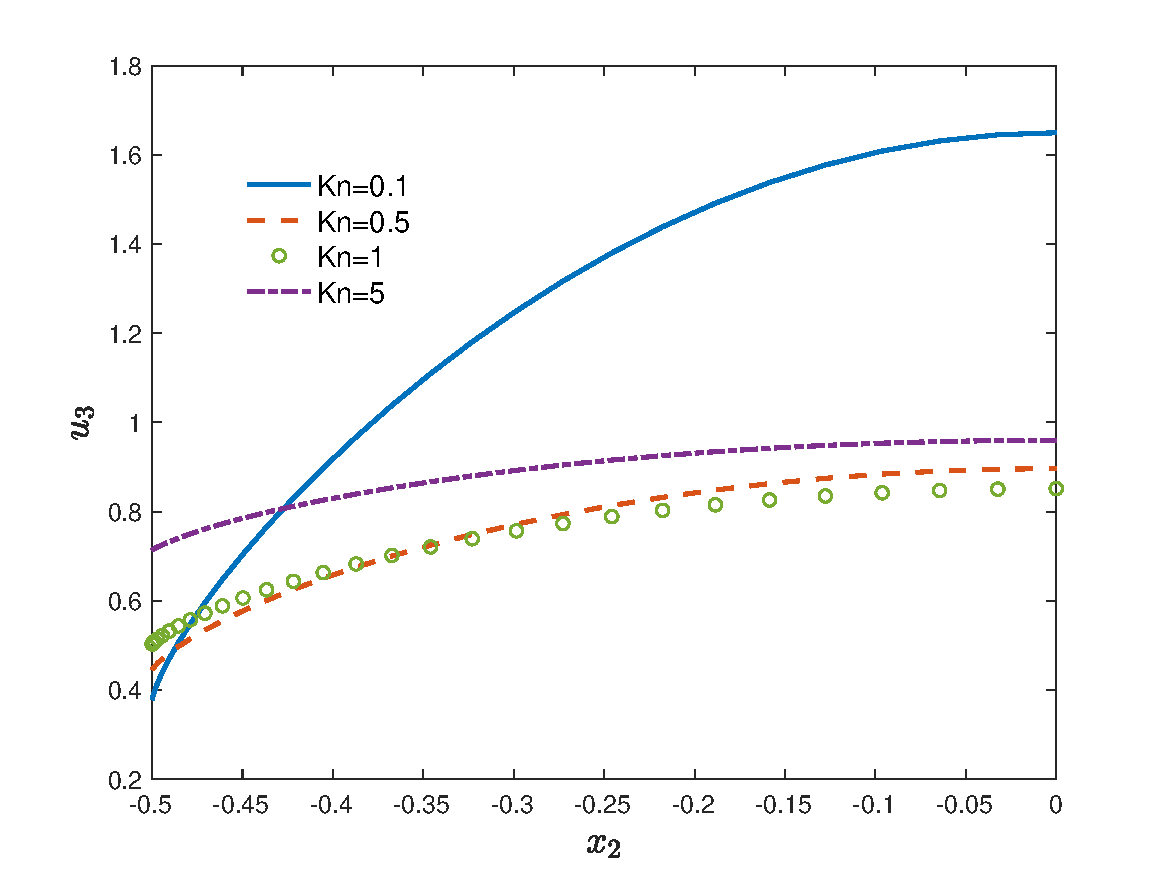
\includegraphics[scale=0.35]{Poiseuille_1D_HS.eps}} 	{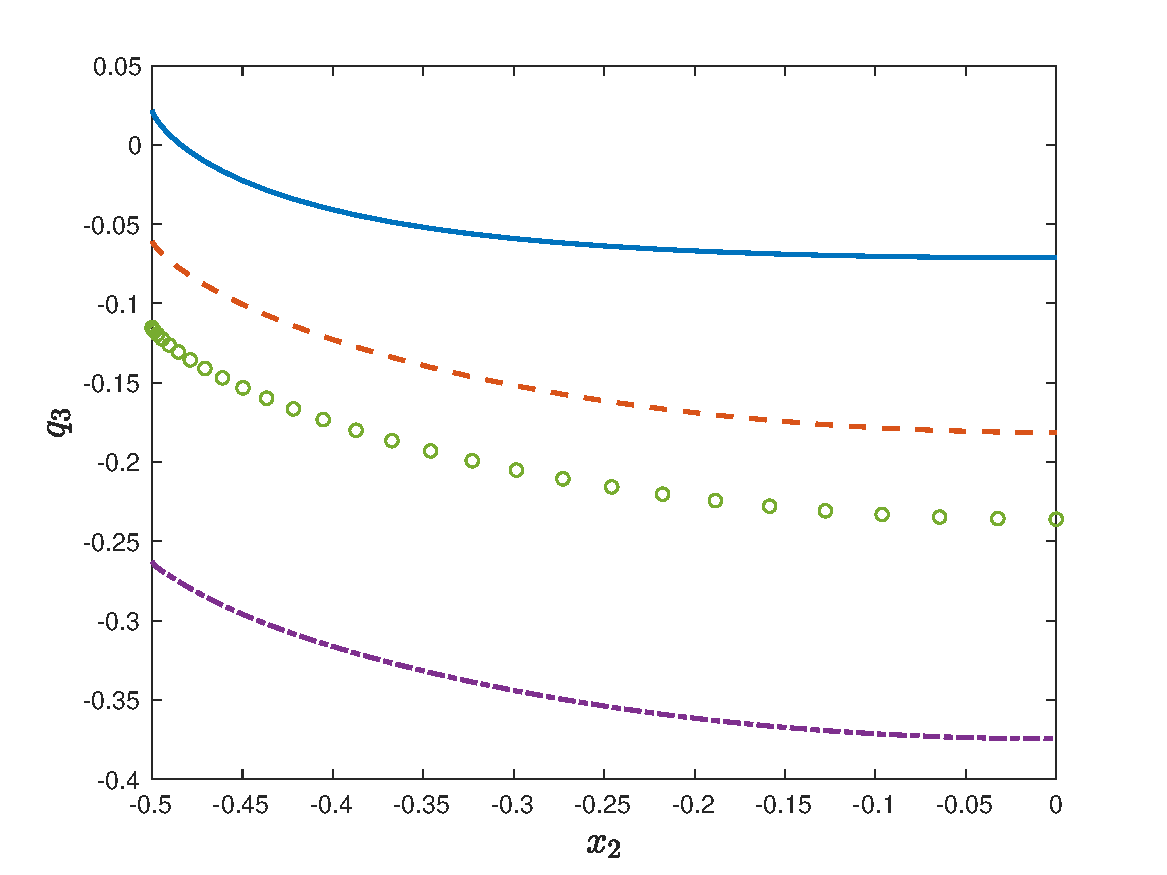
\includegraphics[scale=0.35]{Poiseuille_1D_HS2.eps}}\\
	{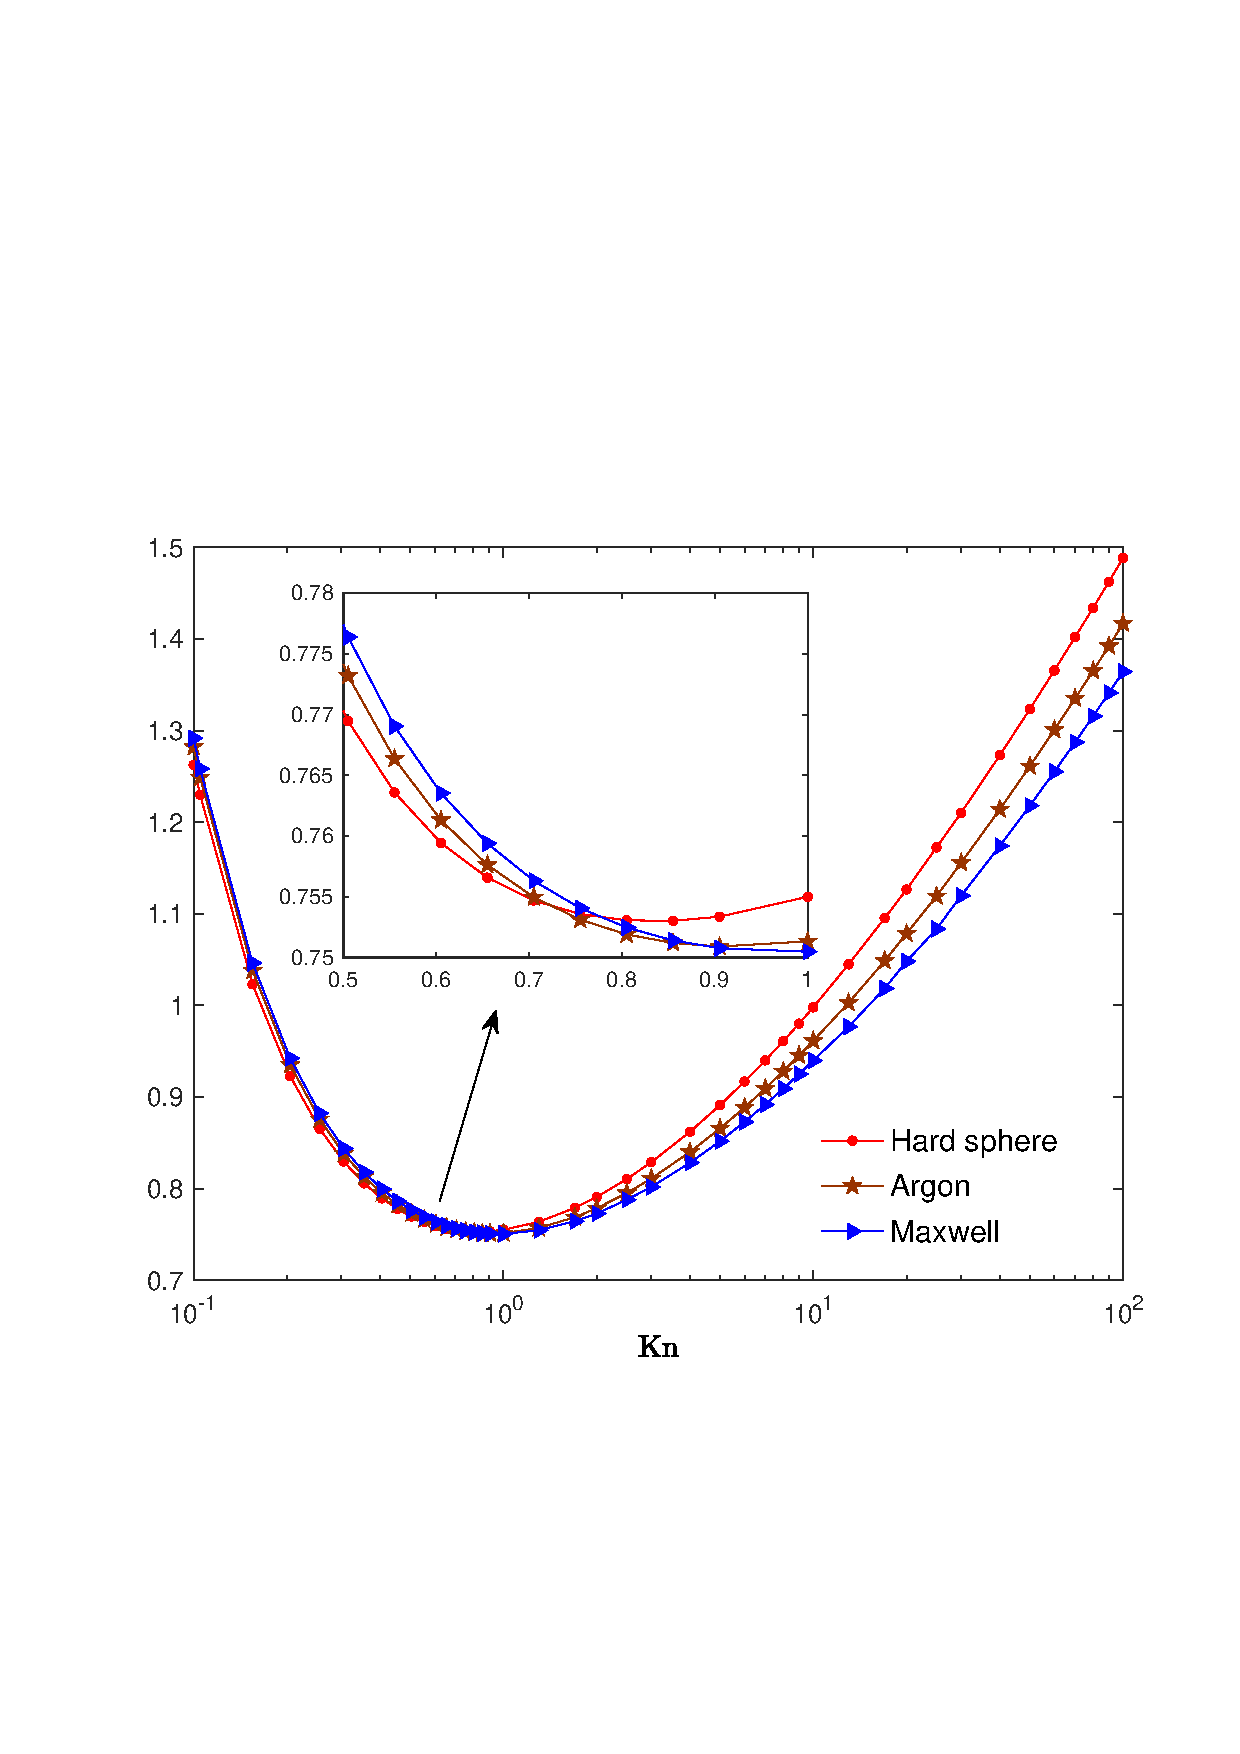
\includegraphics[scale=0.35]{pof_mass.pdf}}\quad
	{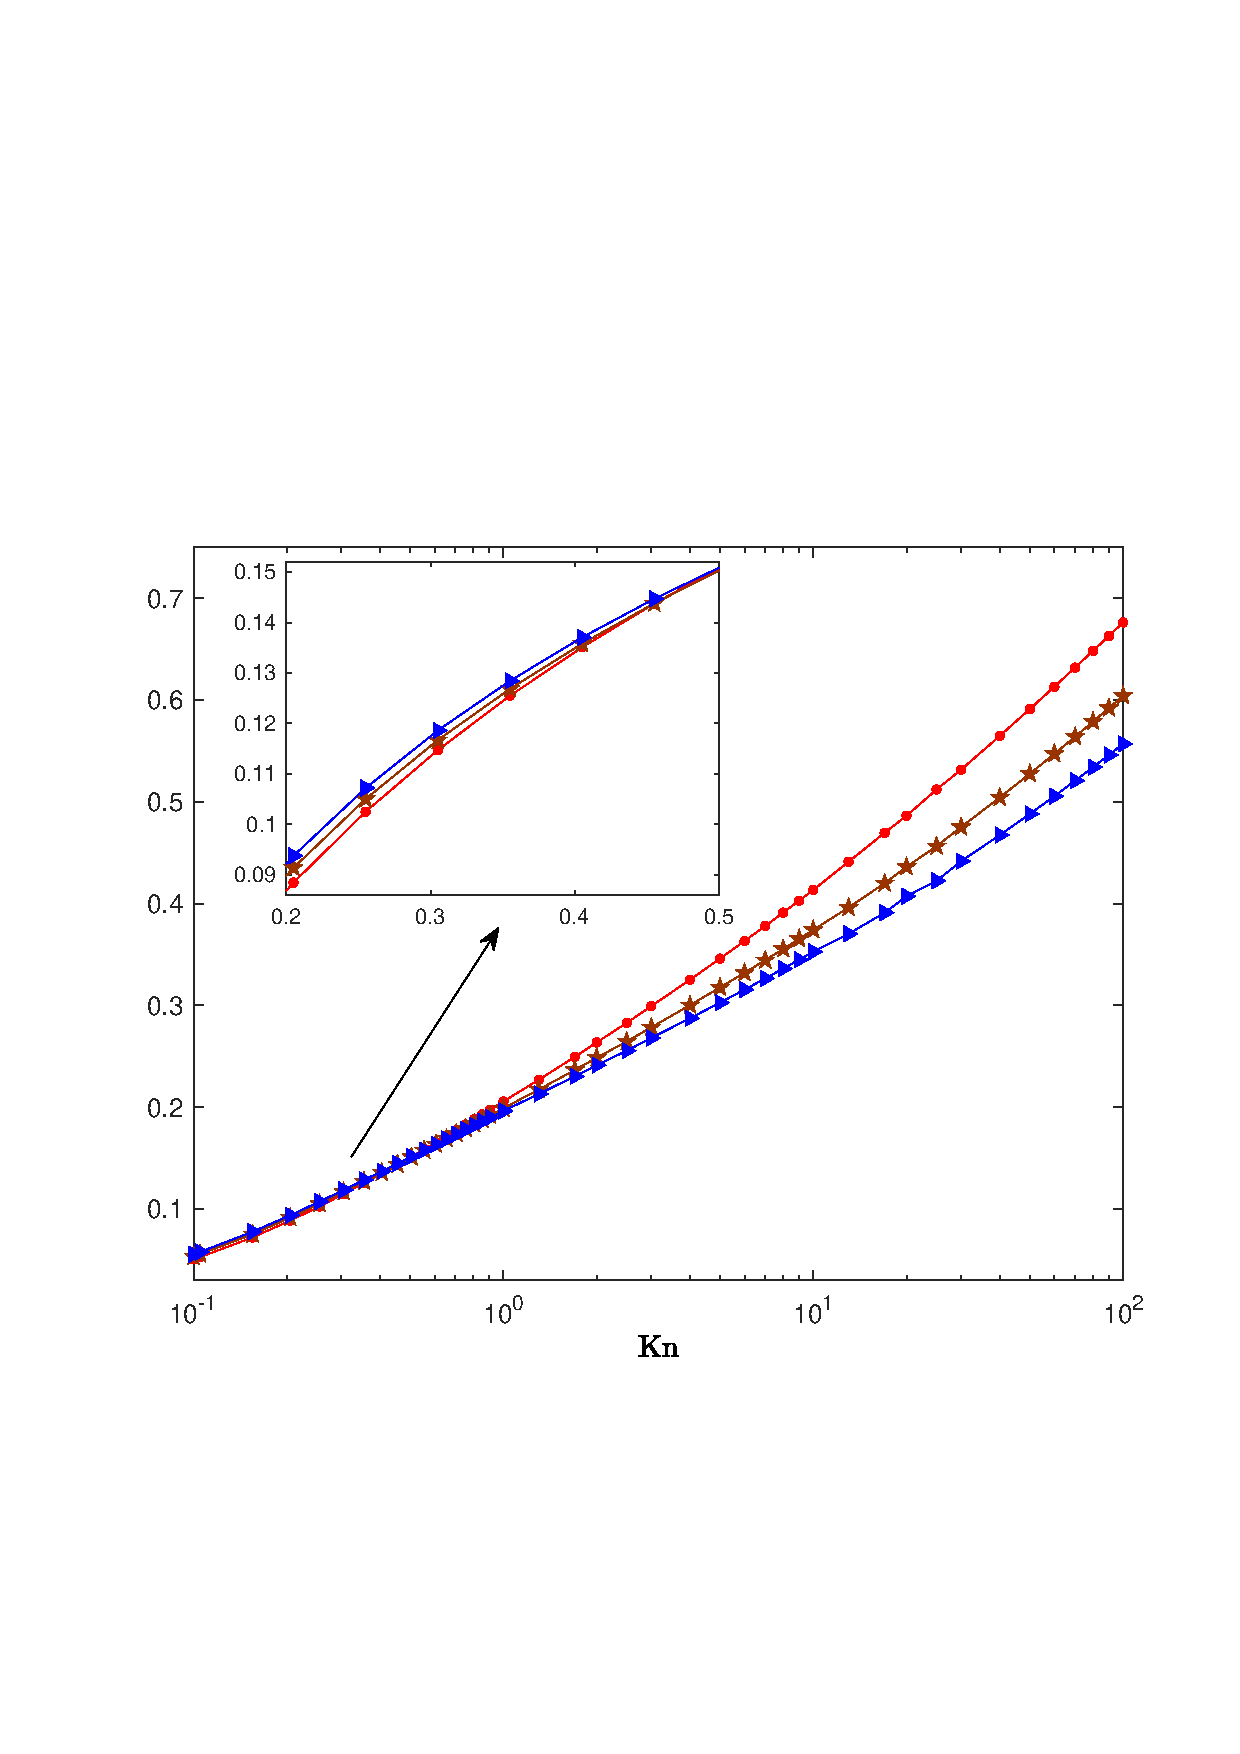
\includegraphics[scale=0.35]{pof_heat.pdf}}
	\caption{ Poiseuille gas flow between parallel plates. (Top row) MFR and HFR in the HS gas. (Bottom row) Comparisons in MFR (left) and HFR (right) for different inverse power-law potentials. The viscosity index for argon is $\omega=0.81$.  } 
	\label{massheat}
\end{figure}


Typical VDF profiles demonstrating the over-concentration phenomena are shown in Fig.~\ref{Onsager0}. When $\text{Kn}=1$, the marginal VDF is roughly proportional to $\exp(-v_2^2)$. However, in the free molecular regime, it can be seen that the marginal VDF has a long tail, and its width shrinks drastically as $1/\text{Kn}$, while its amplitude increases as $\text{Kn}$, which is consistent with the first-order analytical solution of Takata and Funagane~\cite{Takata2011}. 



\begin{figure}[t]
	\centering
	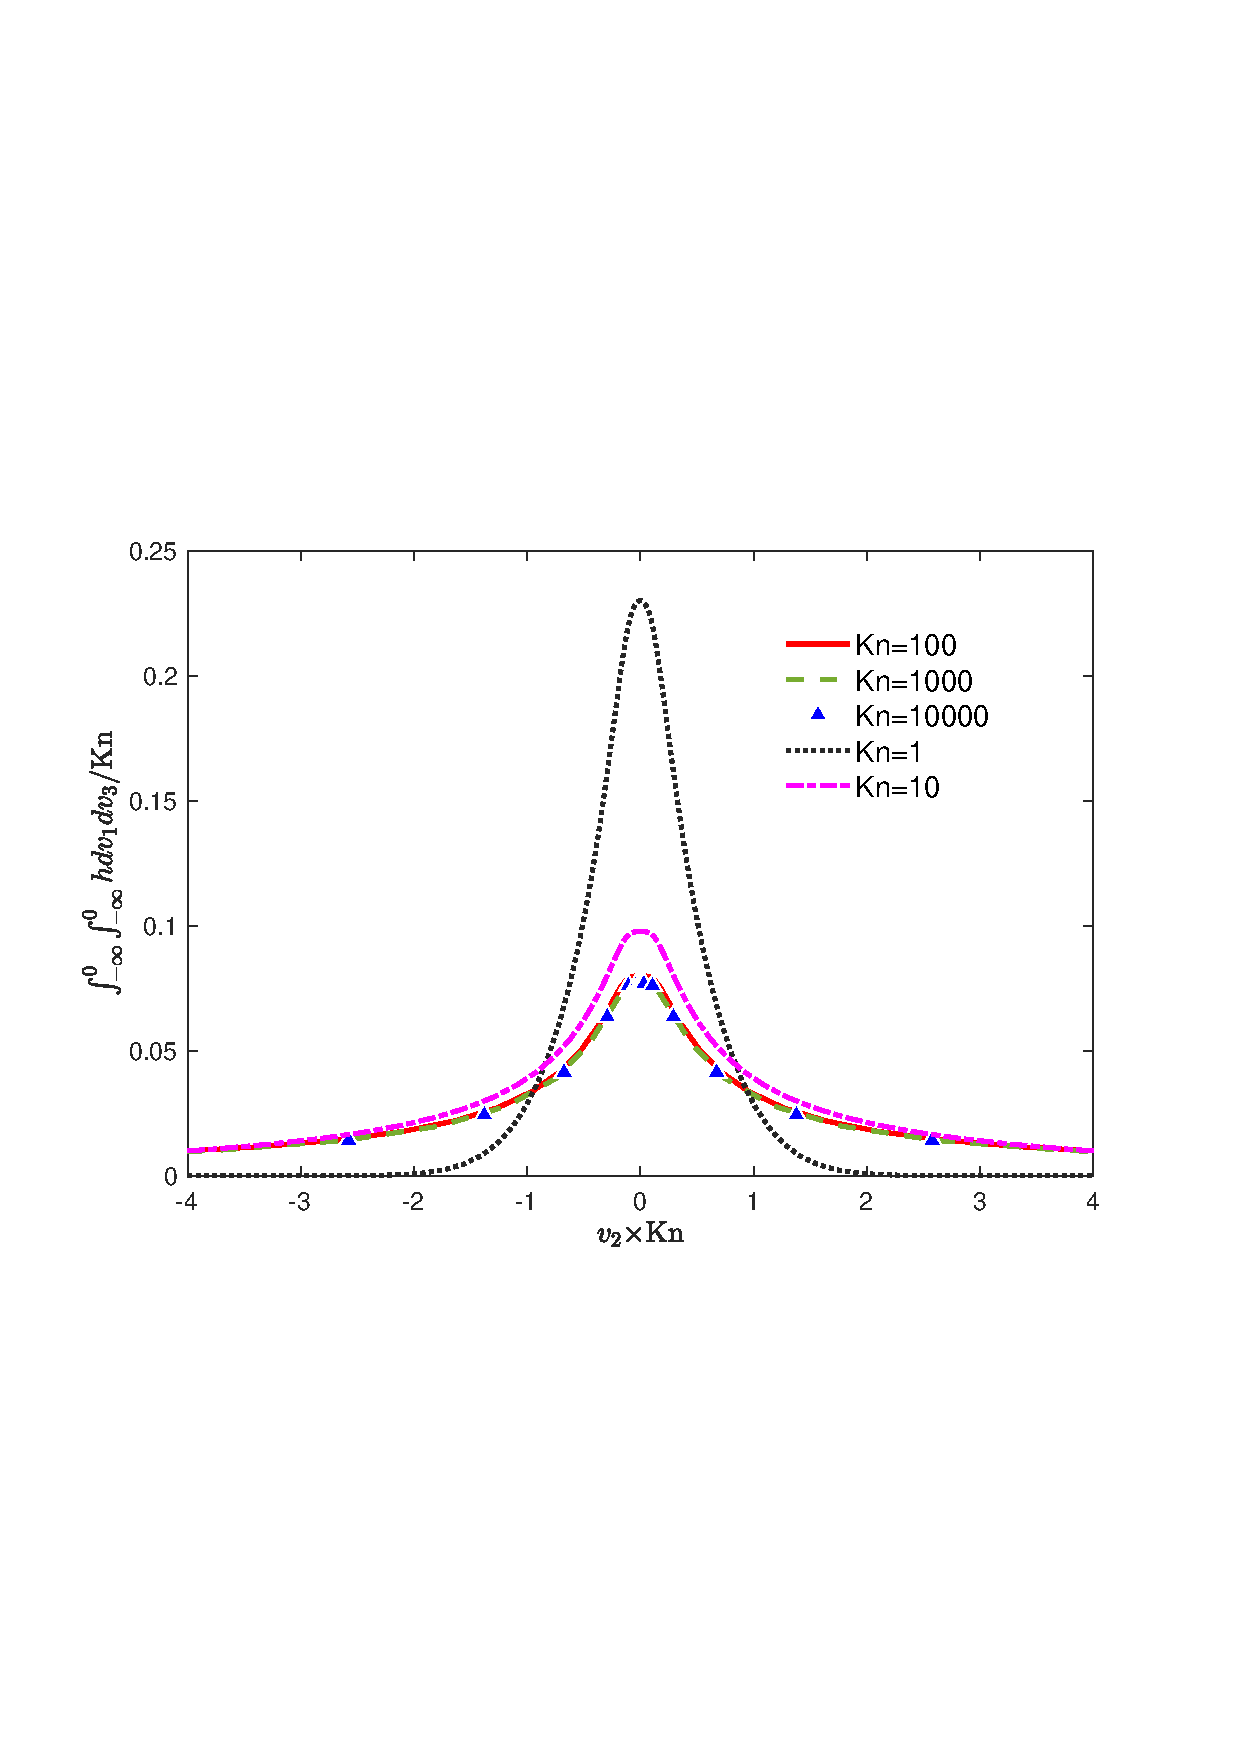
\includegraphics[scale=0.4]{poiseuille_mm.pdf}
    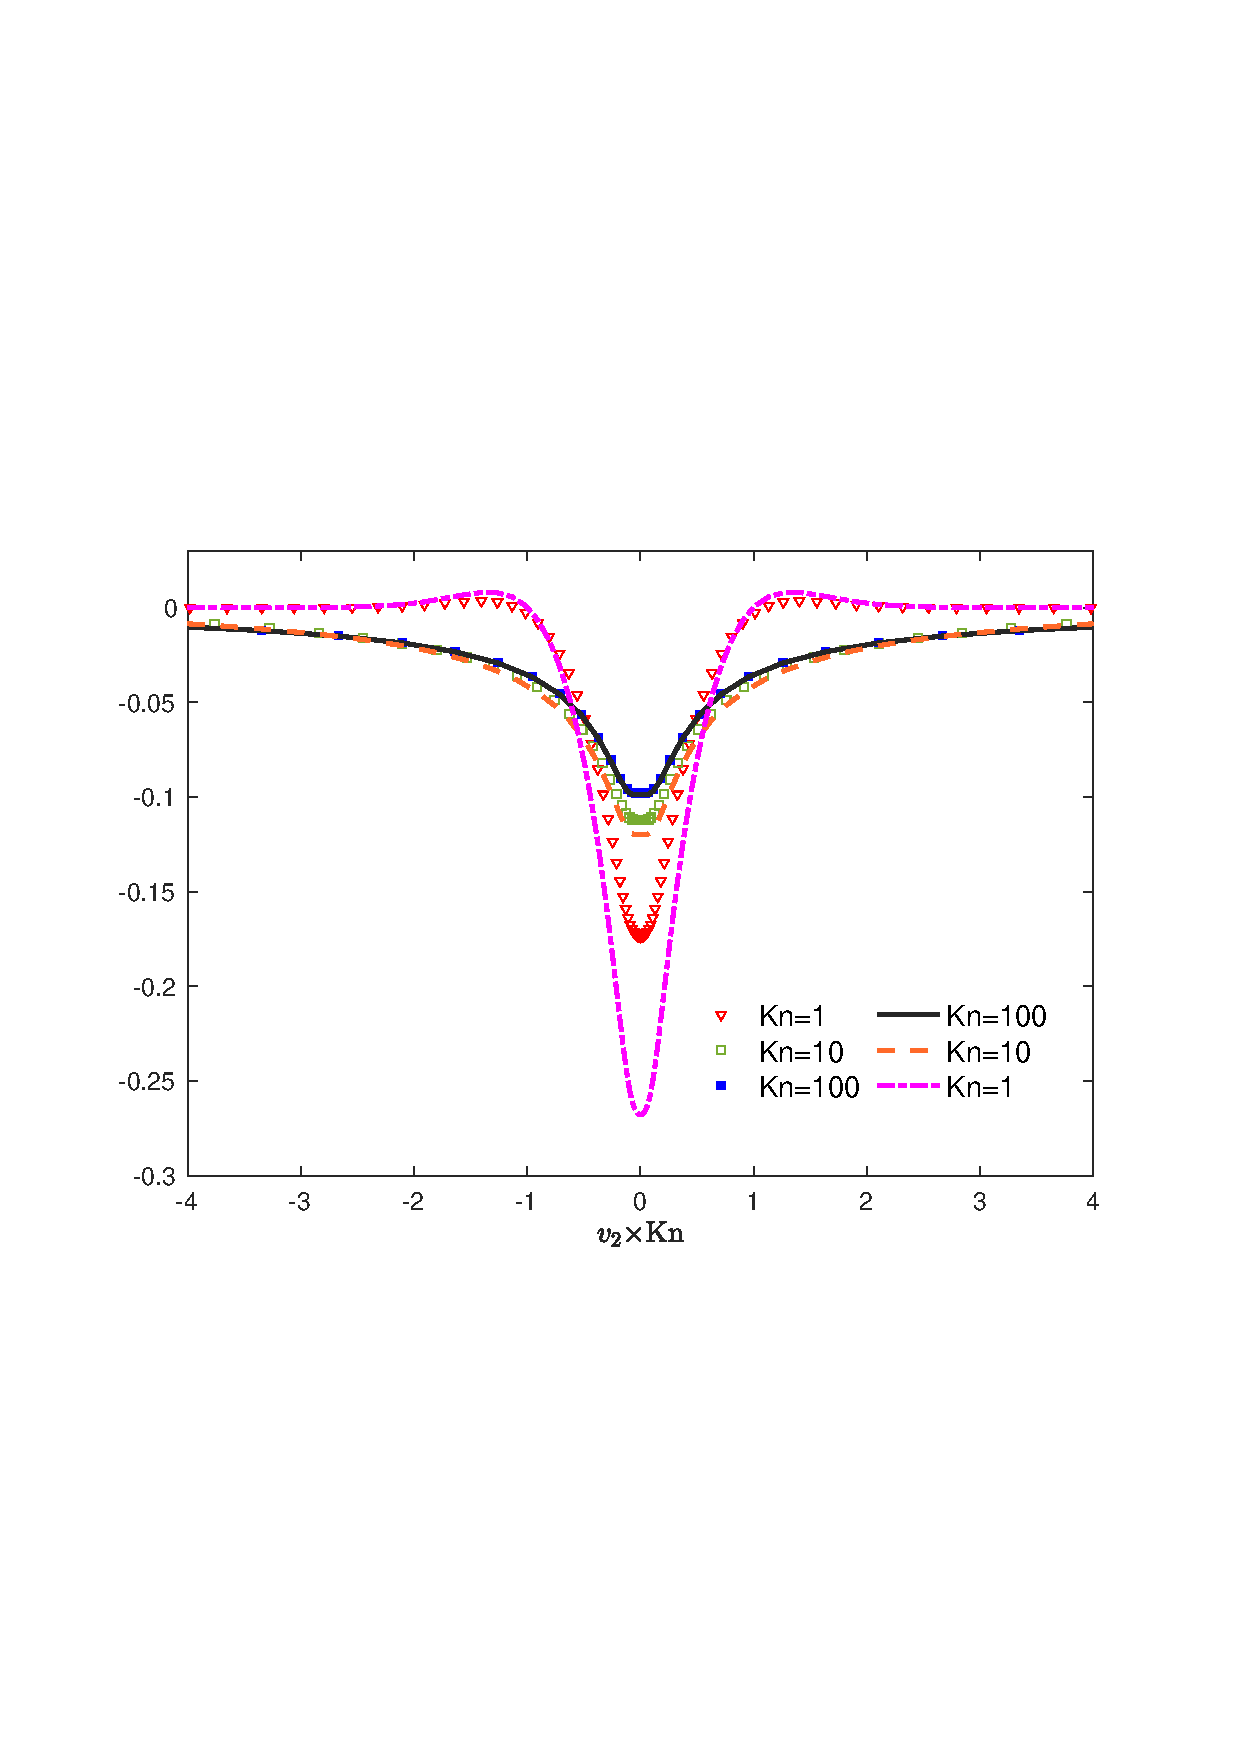
\includegraphics[scale=0.4]{thermal_VDF}
	\caption{ 
		(Left) The marginal VDF in the Poiseuille flow at the channel center. When $\text{Kn}\ge100$, the velocity distribution perpendicular to the plate shrinks as $1/\text{Kn}$, which is known as the ``over-concentration''~\cite{Takata2011}. (Right) 	The Onsager-Casimir relation at the mesoscopic level. Symbols: the marginal VDFs  $\iint_{-\infty}^0{} hdv_1dv_3/\text{Kn}$, where $h$ is obtained in the thermal transpiration. Lines: the marginal VDFs  $\iint_{-\infty}^0{} \left(v^2-\frac{5}{2}\right)hdv_1dv_3/\text{Kn}$, where $h$ is obtained in the Poiseuille flow.
	} 
	\label{Onsager0}
\end{figure}

%\begin{table}[t]
%	\centering
%	\caption{
%		MFR and HFR in the Poiseuille flow of HS gas between two parallel plates.
%	} \label{table_poiseuille_1d_compare} 
%	\begin{tabular}{cccccccccccc}
%		\hline
%		&  \multicolumn{2}{c}{FSM} & \multicolumn{2}{c}
%		{Ohwada \textit{et al.}~\cite{Ohwada_sone_1989}}  &
%		\multicolumn{2}{c}
%		{Takata and Funagane~\cite{Takata2011}} 
%		\\  \hline
%$8\text{Kn}/5\sqrt\pi$ & $G_P$ & $Q_p$ & $G_P$ & $Q_p$ & $G_P$ & $Q_p$\\  
%0.1    & 1.1961 & 0.0552   & 1.1930   & 0.0553  & -      &-  \\  
%0.15   & 0.9951 & 0.0761   & 0.9938   & 0.0761  & -      &-  \\  
%0.2    & 0.9007 & 0.0934   & 0.8999   & 0.0935  & -      &-  \\  
%0.3    & 0.8156 & 0.1208   & 0.8152   & 0.1209  & -      &-  \\  
%0.4    & 0.7804 & 0.1418   & 0.7801   & 0.1419  & -      &-  \\    
%0.6    & 0.7564 & 0.1729   & 0.7562   & 0.1730  & -      &-  \\
%0.8    & 0.7535 & 0.1958   & 0.7533   & 0.1958  & -      &-  \\
%1      & 0.7575 & 0.2140   & 0.7574   & 0.2140  & -      &-  \\
%1.5    & 0.7771 & 0.2477   & 0.7771   & 0.2477  & -      &-\\
%2      & 0.7991 & 0.2724   & 0.7991   & 0.2724  & -      &-\\  
%3      & 0.8399 & 0.3083   & 0.8398   & 0.3082  & -      &-\\
%4      & 0.8750 & 0.3346   & 0.8749   & 0.3345  & -      &-\\
%6      & 0.9322 & 0.3731   & 0.9321   & 0.3730  & -      &-\\
%8      & 0.9779 & 0.4016   & 0.9778   & 0.4015  & -      &-\\
%10     & 1.0160 & 0.4242   & 1.0159   & 0.4242  & 1.0159 & 0.4241  \\
%15 	 & 1.0908 & 0.4669   & 1.0908   & 0.4669  &- 	   &-        \\
%20     & 1.1478 & 0.4984   & 1.1479   & 0.4984  & 1.1477 & 0.4982  \\
%$10^2$ & 1.5143 & 0.6901   & -        &-		  & 1.5143 & 0.6900  \\
%$10^3$ & 2.1210 & 0.9960   & - 		&-		  & 2.1210 & 0.9960  \\
%$10^4$ & 2.7614 & 1.3165   & - 		&-        & 2.7615 & 1.3166  \\  
%$10^5$ & 3.4094 & 1.6405   & - 		&-        & 3.4094 & 1.6406  \\
%$10^6$ & 4.0587 & 1.9652   & - 		&-        & 4.0587 & 1.9652  \\
%		\hline
%	\end{tabular}
%\end{table}



\subsubsection{Poiseuille flow through a long duct}

Consider the Poiseuille flow in a long duct with the aspect ratio $A=S/L$. Unlike the Poiseuille flow between parallel plates where the flow rates increase logarithmically at large $\text{Kn}$, here they saturate at $G_P=\mathcal{M}$ and $Q_P=\mathcal{M}/2$ when $\text{Kn}\rightarrow\infty$~\cite{loyalka1976}, where 
\begin{equation}\label{Mass_flow_rate_fm}
\begin{aligned}[b]
\mathcal{M}=\frac{1}{4\sqrt{\pi}}&\left[\frac{2(A^3+1)}{3A}-\frac{2(A^2+1)^{3/2}}{3A} \right. \\
&\left.
 +\ln\frac{(A^2+1)^{1/2}+A}{(A^2+1)^{1/2}-A}+A\ln\frac{(A^2+1)^{1/2}+1}{(A^2+1)^{1/2}-1} \right].
\end{aligned}
\end{equation}

\begin{table}[t]
	\centering
	\caption{
		MFR and HFR in the Poiseuille flow of HS gas through a rectangular channel. Note that $\text{Kn}=5\pi{}k'/16.$ 
	} \label{table_poiseuille_2d_compare} 
	\begin{minipage}{14cm}
		\centering
		\begin{tabular}{cccccccccccc}
			\hline
			&  \multicolumn{4}{c}{$A=1$} & \multicolumn{4}{c}
			{$A=2$}        \\  
			&  \multicolumn{2}{c}{FSM} & \multicolumn{2}{c}{Doi~\cite{Doi2010}}  
			&  \multicolumn{2}{c}{FSM}    &  \multicolumn{2}{c}{Doi~\cite{Doi2010}}  
			\\  \hline 
			$k'$ & $G_P$ & $Q_P$ & $G_P$ & $Q_P$ & $G_P$ & $Q_P$ & $G_P$ & $Q_P$ \\  
			0.1    & 0.6116 & 0.0445   & 0.613   & 0.045  & 0.9009  & 0.0476    & 0.905   & 0.048\\  
			%0.2    & 0.4691 & 0.0716   & 0.470   & 0.072  & 0.6676  & 0.0790    & 0.668   & 0.079\\  
			0.3    & 0.4260 & 0.0889   & 0.426   & 0.089  & 0.5950  & 0.1013    & 0.595   & 0.101 \\ 
			%0.4    & 0.4066 & 0.1010   & 0.407   & 0.101  & 0.5616  & 0.1175    & 0.562   & 0.118\\  
			0.5    & 0.3960 & 0.1103   & 0.396   & 0.110  & 0.5433  & 0.1301    & 0.544   & 0.130 \\
			%0.6    & 0.3898 & 0.1174   & 0.390   & 0.117  & 0.5322  & 0.1401    & 0.532   & 0.140 \\
			0.8    & 0.3833 & 0.1280   & 0.383   & 0.128  & 0.5203  & 0.1554    & 0.520   & 0.156 \\
			1      & 0.3811 & 0.1356   & 0.381   & 0.136  & 0.5141  & 0.1664    & 0.515   & 0.167 \\
		%	2      & 0.3806 & 0.1558   & 0.380   & 0.156  & 0.5108  & 0.1977    & 0.512   & 0.198\\  
			3      & 0.3835 & 0.1656   & 0.383   & 0.166  & 0.5148  & 0.2131    & 0.516   & 0.214 \\
			%4      & 0.3862 & 0.1717   & 0.386   & 0.172  & 0.5191  & 0.2230    & 0.520   & 0.223 \\
			5      & 0.3886 & 0.1760   & 0.388   & 0.176  & 0.5228  & 0.2300    & 0.523   & 0.230 \\
		%	6      & 0.3906 & 0.1792   & 0.390   & 0.179  & 0.5261  & 0.2352    & 0.527   & 0.236 \\
			8      & 0.3938 & 0.1837   & 0.394   & 0.184  & 0.5314  & 0.2428    & 0.532   & 0.243  \\
			10     & 0.3963 & 0.1869   & 0.396   & 0.187  & 0.5354  & 0.2481    & 0.536   & 0.248  \\
			20     & 0.4033 & 0.1948   & -       &-       & 0.5479  & 0.2613    & -       & -  \\
			50     & 0.4102 & 0.2016   & -       &-       & 0.5596  & 0.2734    & -       & -  \\
			$10^2$ & 0.4136 & 0.2048   & -       &-       & 0.5657  & 0.2791    & -       & -  \\
			$10^3$ & 0.4183 & 0.2089   & -       &-       & 0.5742  & 0.2865    & -       & - \\   
			$10^4$ & 0.4191 & 0.2095   & -       &-       & 0.5758  & 0.2878    & -       & - \\   
			$\infty$\footnote{Data in columns 4, 5, 8, and 9 are obtained from Eq.~\eqref{Mass_flow_rate_fm}.} & 0.4194 & 0.2097   & 0.4194  & 0.2097 & 0.5762  & 0.2881    & 0.5762  & 0.2881  \\
			\hline
		\end{tabular}\par
		\vspace{-0.75\skip\footins}
		\renewcommand{\footnoterule}{}
	\end{minipage}
\end{table}


This problem was first solved by the numerical kernel method and then by the low-variance DSMC for HS molecules~\cite{Doi2010,Radtke2011}. Nice agreement in the mass and heat flow rates with Doi's are shown in Table~\ref{table_poiseuille_2d_compare}. 


%To compare the numerical efficiency with the low-variance DSMC, we consider the HS gas inside a square channels; with a $25\times25$ spatial cell mesh, $32\times32\times24$ frequency components, and $M=6$, we obtain $G_P=0.3808$ and 0.3966,  $Q_P=0.1365$ and 0.1874 for $\text{Kn}_{vhs}=1$ and 10, respectively, compared to Doi's 0.381 and 0.396 for $G_P$, and 0.136 and 0.187 for $Q_P$. The computational time is about 1 minute, compared to the low-variance DSMC that takes respectively 66 and 12 minutes. %Note that our Fortran program runs on a single core of an Intel Q9650 (3.0 GHz Core 2 Quad processor). 
%The time is obtained when there is 0.1\% statistical uncertainty in MFR. To achieve the same level of uncertainty in the velocity field, the low-variance DSMC would need 240 and 120 minutes, respectively. %These comparisons indicate that the FSM is accurate and efficient.

%.\footnote{With the general synthetic iterative scheme in Chapter~\ref{chap:GSIS}, we can achieve the efficiency for any value of Knudsen number, while the simulation time for conventional iterative scheme and low-variance DSMC increases dramatically when $Kn$ decreases.}. 



\section{Thermal transpiration}
\label{poiseuille_dis}
\index{thermal transpiration}


Thermal transpiration, where the gas moves towards a hotter region even in the absence of a pressure gradient~\citep{Reynolds1879,Maxwell1879vii}, is one of the fundamental problems in rarefied gas dynamics. It has found applications in many engineering problems, including the Crookes radiometer~\cite{crookes1874xv}, the Knudsen compressor that pumps the gas without any moving mechanical part~\citep{vargo1999knudsen,gupta2008thermal}, the capacitance diaphragm gauge where the effects of thermal transpiration should be subtracted for accurate measurement of low gas pressures~\citep{Sentina1999,Daude2014Vacuum}, gas mixture separation~\citep{Takata2007EJMB}, and the Leidenfrost ratchet which rectifies the vapor flow in the boundary layer~\citep{wurger2011leidenfrost}. Thermal transpiration arises when the Knudsen number becomes appreciable in micro/nano-devices and/or low-pressure environments.


In thermal transpiration, the gas pressure is maintained constant, while the wall temperature varies linearly in the $x_3$ direction as
\begin{equation}
T=T_0\left(1+\beta_T\frac{x_3}{L}\right), \quad
\beta_T=\frac{L}{T_0}\frac{dT}{dx_3},
\end{equation} 
where the dimensionless temperature gradient $\beta_T$ is very small. The Boltzmann equation can be linearized around the equilibrium state, when $h$ in Eq.~\eqref{Chapter_lin_VDF} is replaced by $h+x_3f_{eq}({v}^2-\frac{5}{2})$, resulting 
\begin{equation}\label{thermal_tube}
v_1\frac{\partial h}{\partial x_1}+v_2\frac{\partial h}{\partial x_2}=\mathcal{L}^+(h)-\nu_{eq}{h}-{v_3}\left({v}^2-\frac{5}{2}\right)f_{eq}.
\end{equation}


The MFT and HFR are expressed as
\begin{equation}\label{normalized_MFR_thermal}  
\begin{aligned}[b]
\dot{M}&=\frac{2p_0S}{v_m}\beta_TG_T, \quad  G_T=\frac{1}{A}\iiint {v_3h}dx_1dx_2d\bm{v}, \\
\dot{E}&=-p_0v_mS\beta_T{}Q_T, \quad   Q_T=-\frac{1}{A}\iiint {\left({v}^2-\frac{5}{2}\right)v_3}hdx_1dx_2d\bm{v}.
\end{aligned}
\end{equation}







\begin{table}[t]
	\centering
	\caption{MFR and HFR in the thermal transpiration of HS gas through a rectangular channel. Note that $\text{Kn}=5\pi{}k'/16$.} \label{table_thermal_2d_compare} 
	\begin{minipage}{14cm}
		\centering
		\begin{tabular}{cccccccccccc}
			\hline
			&  \multicolumn{4}{c}{$A=1$} & \multicolumn{4}{c}
			{$A=2$}        \\  
			&  \multicolumn{2}{c}{FSM} & \multicolumn{2}{c}{Ref.~\cite{Doi2010}}  
			&  \multicolumn{2}{c}{FSM}    &  \multicolumn{2}{c}{Ref.~\cite{Doi2010}}  
			\\  \hline 
			$k'$ & $G_T$ & $Q_T$ & $G_T$ & $Q_T$ & $G_T$ & $Q_T$ & $G_T$ & $Q_T$ \\  
			0.1    & 0.0450 & 0.1759  & 0.045  & 0.176   & 0.0479 & 0.1842 & 0.048  & 0.185  \\  
		%	0.2    & 0.0719 & 0.2936  & 0.072  & 0.294   & 0.0793	& 0.3199 & 0.079  & 0.320  \\  
			0.3    & 0.0891 & 0.3748  & 0.089  & 0.375   & 0.1014 & 0.4205 & 0.101  & 0.421  \\ 
		%	0.4    & 0.1012 & 0.4341  & 0.102  & 0.434   & 0.1176	& 0.4976 & 0.118  & 0.498  \\  
			0.5    & 0.1103 & 0.4794  & 0.110  & 0.479   & 0.1302 & 0.5587 & 0.130  & 0.560  \\
		%	0.6    & 0.1174 & 0.5153  & 0.118  & 0.514   & 0.1403 & 0.6085 & 0.140  & 0.609  \\
			0.8    & 0.1279 & 0.5690  & 0.128  & 0.568   & 0.1556 & 0.6852 & 0.155  & 0.686  \\
			1      & 0.1356 & 0.6077  & 0.136  & 0.606   & 0.1668	& 0.7433 & 0.167  & 0.743  \\
		%	2      & 0.1560 & 0.7098  & 0.156  & 0.708   & 0.1980 & 0.9003 & 0.198  & 0.900  \\  
			3      & 0.1658 & 0.7571  & 0.166  & 0.756   & 0.2135 & 0.9762 & 0.214  & 0.976  \\
		%	4      & 0.1719 & 0.7856  & 0.172  & 0.784   & 0.2233 & 1.0229 & 0.223  & 1.023  \\
			5      & 0.1761 & 0.8052  & 0.176  & 0.804   & 0.2303 & 1.0553 & 0.230  & 1.055  \\
		%	6      & 0.1793 & 0.8197  & 0.179  & 0.818   & 0.2355 & 1.0795 & 0.236  & 1.079  \\
			8      & 0.1839 & 0.8399  & 0.184  & 0.839   & 0.2431 & 1.1136 & 0.243  & 1.113  \\
			10     & 0.1870 & 0.8536  & 0.187  & 0.852   & 0.2484 & 1.1370 & 0.248  & 1.136  \\
			20     & 0.1950 & 0.8867  & -      &-        & 0.2618 & 1.1942 & -      & -      \\
			50     & 0.2017 & 0.9138  & -      &-        & 0.2736 & 1.2420 & -      & -      \\
			$10^2$ & 0.2048 & 0.9258  & -      &-        & 0.2792 & 1.2636 & -      & -      \\
			$10^3$ & 0.2089 & 0.9406  & -      &-        & 0.2866 & 1.2909 & -      & -      \\   
			$10^4$ & 0.2095 & 0.9430  & -      &-        & 0.2878 & 1.2954 & -      & -      \\   
			$\infty$\footnote{Data in columns 4, 5, 8, and 9 are obtained from Eq.~\eqref{Mass_flow_rate_fm}.} & 0.2097 & 0.9436  & 0.2097 & 0.9436  & 0.2881 & 1.2965 & 0.2881 & 1.2965 \\
			\hline
		\end{tabular}\par
		\vspace{-0.75\skip\footins}
		\renewcommand{\footnoterule}{}
	\end{minipage}
\end{table}


\begin{figure}[t]
	\centering
	{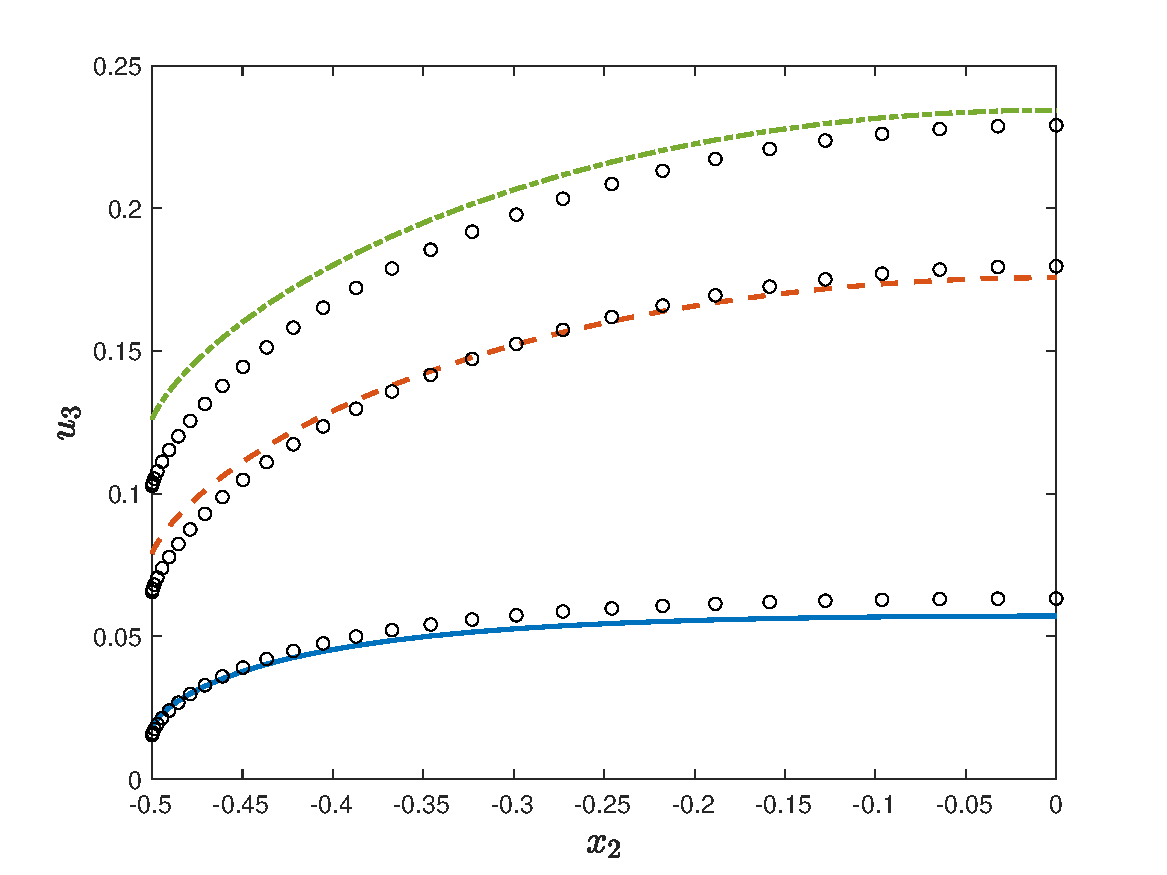
\includegraphics[scale=0.4]{Transpiration_1D.eps}} 	{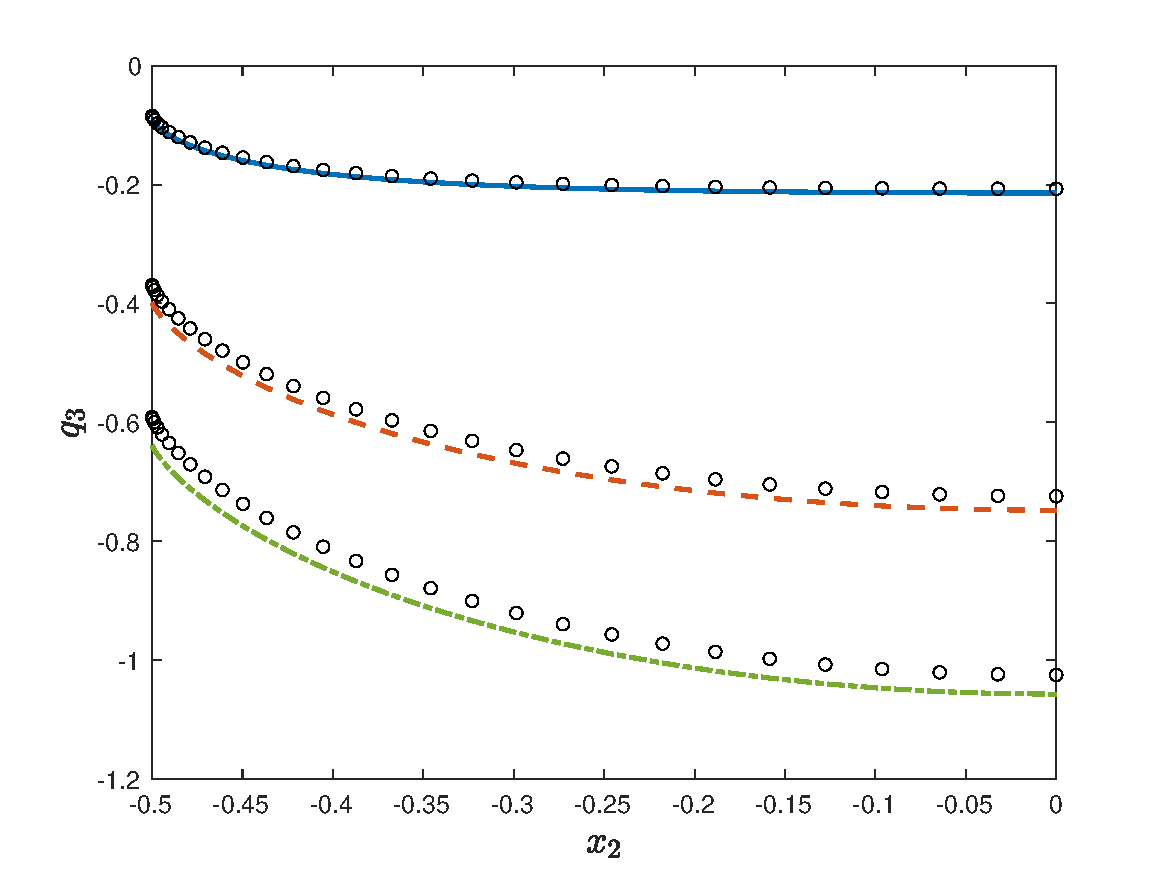
\includegraphics[scale=0.4]{Transpiration_1D2.eps}}
	\caption{ Profiles of velocity and heat flux in the thermal transpiration between two parallel plates. Solid, dashed, dash-dotted lines are the results of HS gas, when $\text{Kn}=0.1$, 0.5, and 1, respectively, while circles are the corresponding results of Maxwell gas.   } 
	\label{Transpiration_massheat}
\end{figure}


Profiles velocity and heat flux are shown in Fig.~\ref{Transpiration_massheat}, whose magnitudes increase with the Knudsen number. Again, it is observed that although the Knudsen number is the same, different intermolecular potential (viscosity index) has different macroscopic profiles.



For the rectangular cross-section, the mass flow rate is $G_T=\mathcal{M}/{2}$ and the heat flow rate in the free-molecular flow regime~\cite{loyalka1976} is $G_T={9}\mathcal{M}/4$, where $\mathcal{M}$ is given by Eq.~\eqref{Mass_flow_rate_fm}. The comparison in MFR and HFR with Doi's results are shown in Table~\ref{table_thermal_2d_compare}, where good agreements can be found.



\subsubsection{Onsager-Casimir relation}
%\begin{figure}[t]
%	\centering
%	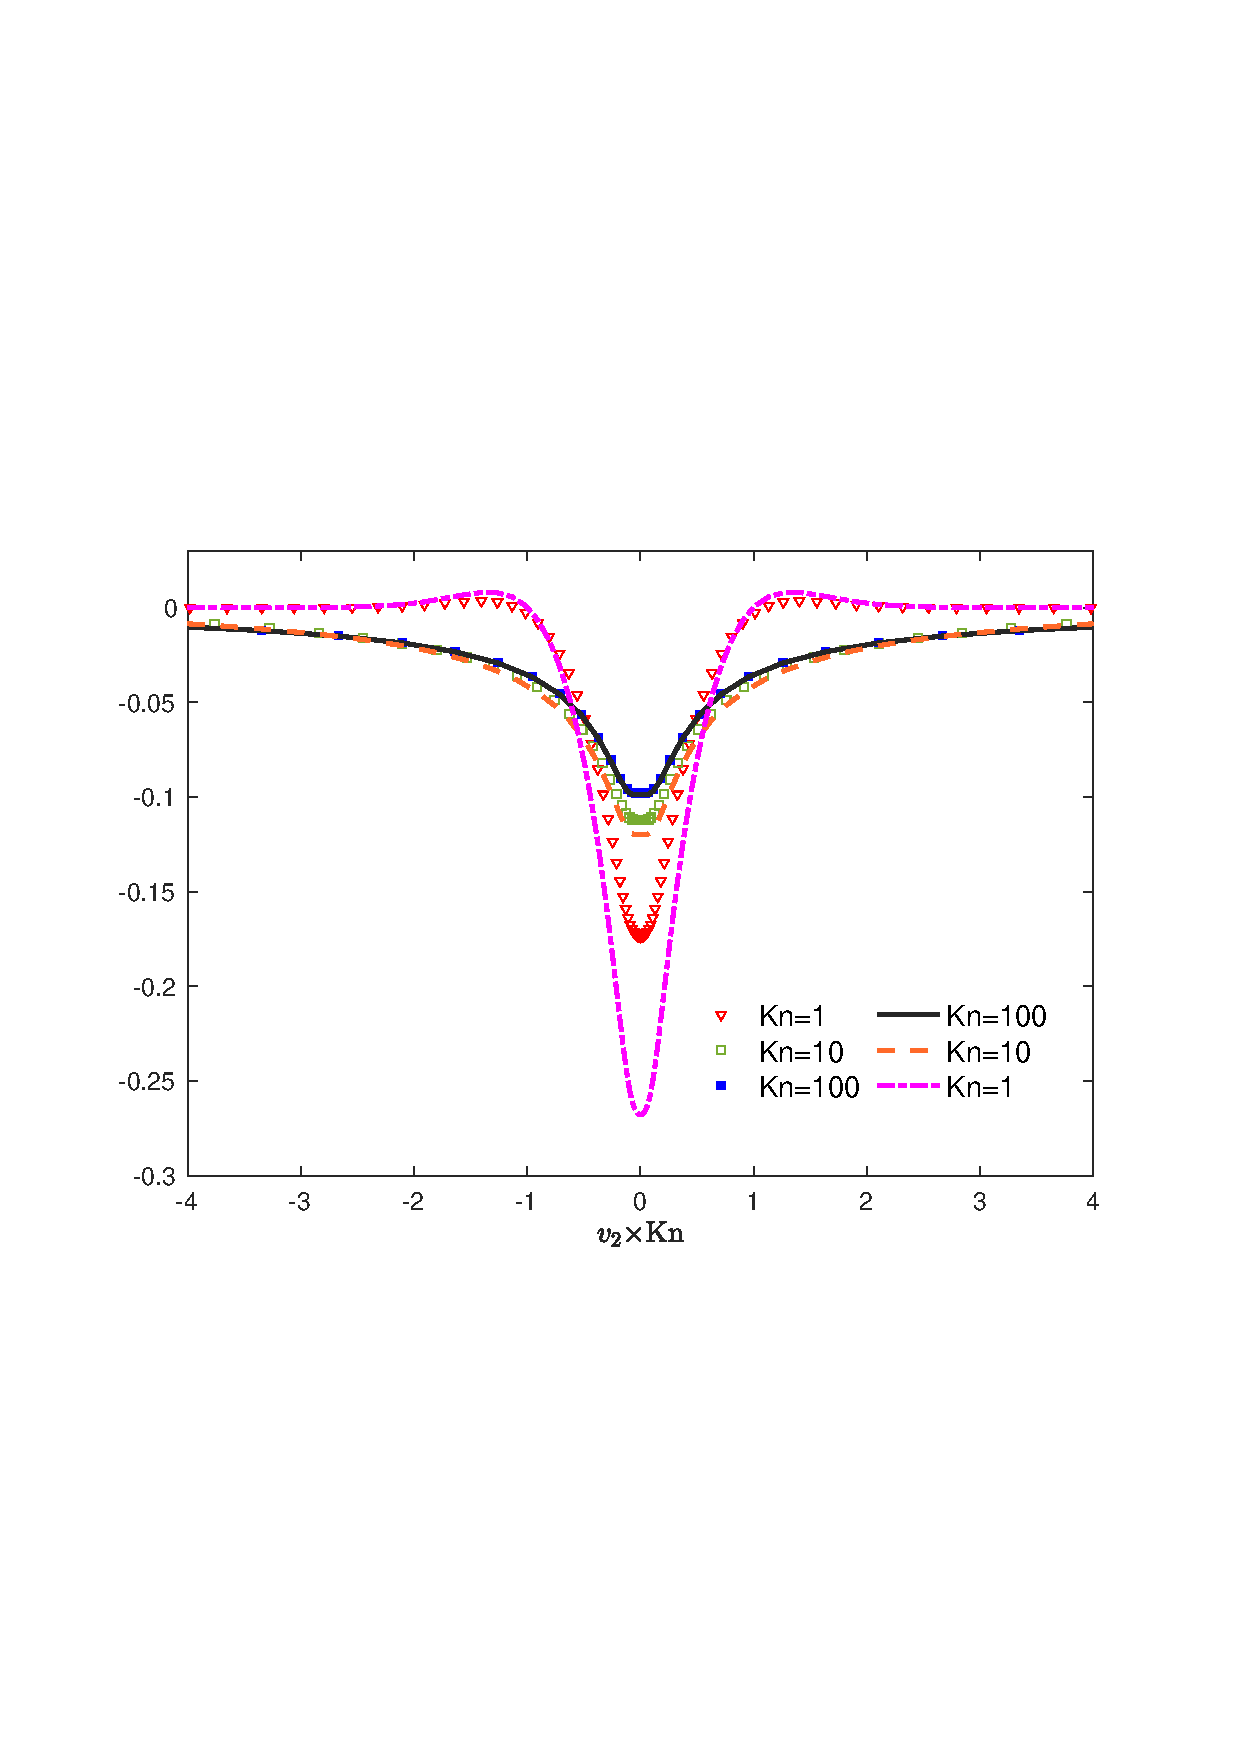
\includegraphics[scale=0.5]{thermal_VDF}
%	\caption{ 
%		The Onsager-Casimir relation at the mesoscopic level. Symbols: the marginal VDFs  $\iint_{-\infty}^0{} hdv_1dv_3/\text{Kn}$, where $h$ is obtained in the thermal transpiration. Lines: the marginal VDFs  $\iint_{-\infty}^0{} \left(v^2-\frac{5}{2}\right)hdv_1dv_3/\text{Kn}$, where $h$ is obtained in the Poiseuille flow.
%	} 
%	\label{Onsager}
%\end{figure}


The Onsager-Casimir relation states that the MFR in the thermal transpiration is equal to the heat flow rate in the Poiseuille flow. In the numerical simulation we find that this relation is held with the absolute error smaller than $10^{-4}$. Takata and Funagane~\cite{Takata2011} made the important observation that at large $\text{Kn}$, $u_3[h_T]$ and $q_3[h_P]$ are even identical at the level of spatial profile:
\begin{equation}
u_3[h_T]=q_3[h_P]+O\left(\frac{(\ln{\text{Kn}})^2}{\text{Kn}}\right).
\end{equation}
Our numerical results in Fig.~\ref{Onsager0} further show that the agreement is even at the mesoscopic level:
\begin{equation}
h_T\approx\left({v}^2-\frac{5}{2}\right)h_P.
\end{equation} 

%
%The asymptotic mass flow rates at large $\text{Kn}$ in the Poiseuille flow and thermal transpiration have also been obtained~\cite{Takata2011}. It has been found that they increase logarithmically with respect to $\text{Kn}$. For the heat flow rate in the thermal transpiration, we find it can also be well fitted by the logarithmic function of $\text{Kn}$:
%\begin{equation}
%Q_T=0.6345\ln(\text{Kn})+Q_0
%\end{equation} 
%in the region $10^5<\text{Kn}<2\times10^6$, where the constant $Q_0$ is 0.2679, 0.1762, 0.07371, and -0.09903 for the HS molecules, helium, argon, and the Maxwell molecules, respectively.



\section{Influence of intermolecular potential}

It should be noted that except for the HS gas, the collision kernels in the previous  chapter are all modeled to recover the shear viscosity, rather than calculated directly from intermolecular potential. Then it is natural to ask does the effects of intermolecular potential, observed in Figs.~\ref{massheat} and \ref{Transpiration_massheat}, exist when the exact collision kernel for realistic intermolecular potentials is used? To this end, we extend the FSM to solve the LBE with the Lennard-Jones potential~\eqref{Lennard_Jones_chapter}. 


\subsection{Collision kernel from Lennard-Jones potential}\label{linear_LJ_FSM}

When the Lennard-Jones potential is considered, the LBE remains unchanged. However, the collision kernel $B(\theta,v_r)$ in Eqs.~\eqref{linearized1} and~\eqref{linearized2} becomes~\cite{wuPoF2015}:
\begin{equation}\label{LJ_collision_kernel}
B(\theta,v_r)=(n_0d_{LJ}^2L)\sigma_Dv_r,
\end{equation} 
where the differential cross-section, after the Carleman representation, is
\index{differential cross-section}
\begin{equation}
\sigma_D=\sigma_D\left(2\text{arctan}\frac{|y|}{|z|},v_m\sqrt{y^2+z^2}\right)\equiv\sigma_D'(|y|,|z|).
\end{equation}
In general, $y$ and $z$ in $\sigma_D'(|y|,|z|)$ cannot be separated as $\sigma_1(|y|)\sigma_2(|z|)$, and the kernel mode 
$\beta(\bm{l},\bm{m})$ can only be simplified to
\begin{equation}\label{kernel_LJ_mode00}
\begin{aligned}[b]
\beta(\bm{l},\bm{m})=&(n_0d_{LJ}^2L)\iint {}d\bm{e}'d\bm{e} \delta(\bm{e}\cdot{\bm{e}'})\\
\times&
\int_{-R}^R\int_{-R}^R|\rho\rho'|\sigma'_D(|\rho|,|\rho'|)\exp(i\rho\xi_{\bm{l}}\cdot{\bm{e}}+i\rho'\xi_{\bm{m}}\cdot{\bm{e}'})d\rho d\rho'.
\end{aligned}
\end{equation}



To enable the FFT-based convolution, the integration with respect to $\rho$ is approximated by a numerical quadrature~\cite{Hu2012,wuPoF2015}, such that the integration with respect to $\rho'$ can be calculated accurately, or vise versa. Suppose $\rho_r$ and $\omega_r$ with $r=1,2,\cdots,M_r$ are the abscissas and weights of a quadrature in the region $[0,R]$, Eq.~\eqref{kernel_LJ_mode00} becomes\footnote{For the Lennard-Jones potential, for each relative collision energy $E$, the differential cross-section is a continuous function of the deflection angle at $E=u^2k_BT_0/(2\epsilon)=(\rho_r^2+\rho'^2)k_BT_0/(2\epsilon)\lesssim1$ and has one discontinuous point at $E>1$~\cite{Sharipov_trans}. Therefore, the integration region $0\le\rho\le{}R$ is divided into two regions: the first region $[0,\sqrt{2\epsilon/k_BT_0}]$ is divided into 9 uniform sections, while the second region $[\sqrt{2\epsilon/k_BT_0},R]$ is discretized according to the Gauss-Legendre quadrature of order 7. So the number of points in the discretization of  $\rho$ is $M_r=16$.} 
\begin{equation}
\beta(\bm{l},\bm{m})=(n_0d_{LJ}^2L)\sum_{r}\omega_r\iint  \delta(\bm{e}\cdot{\bm{e}'})\phi(\rho_r,\xi_{\bm{l}}\cdot{\bm{e}})\psi(\rho_r,\xi_{\bm{m}}\cdot{\bm{e}'})d\bm{e}'d\bm{e},
\end{equation} 
where $\psi(\rho_r,s)=2\int_0^R \rho'\sigma'_D(\rho_r,\rho')\cos(\rho's) d\rho'$ and $\phi(\rho_r,s)=2\rho_r\cos(\rho_rs)$. Then, following the straightforward algebraic calculation in Chapter~\ref{fourier_galerkin_spectral}, we have
\begin{equation} \label{kernel_modee}
\beta(\bm{l},\bm{m})= 4(n_0d_{LJ}^2L)\sum_{p,q,r=1}^{M,M,M_r}{\omega_p\omega_q\omega_r}
\phi(\rho_r,\xi_{\bm{l}}\cdot{\bm{e}_{\theta_p,\varphi_q}}) 
\psi'\left(\rho_r,\xi^\perp_{\bm{l}}\
\right) \sin\theta_p,
\end{equation}
where\footnote{We first check the continuity of the differential cross-section as $\rho'$ goes from 0 to $R$. If $\sigma'_D(\rho_r,\rho')$ is continuous, then Eq.~\eqref{psi_expression} is approximated by the Gauss-Legendre quadrature of order 120. Otherwise, suppose $\sigma'_D(\rho_r,\rho')$ is discontinuous at $\rho'=\rho'_d$, then the region $\rho'\in[0,\rho'_d)$ is discretized non-uniformly by 60 points, with most of the points located near $\rho'_d$, while the remaining region $\rho'\in[\rho'_d,R]$ is approximated by the Gauss-Legendre quadrature of order 60. In the numerical integration of $\psi'$, a differential cross-section with deflection angle less than 0.05 radians is neglected. Finally, when $\psi'\left(\rho_r,s\right)$ is obtained, $\psi'\left(\rho_r,\xi^\perp_{\bm{l}}\right)$ is calculated through cubic interpolation. } 
\begin{equation}\label{psi_expression}
\psi'(\rho_r,s)=2\pi\int_0^R \rho'\sigma'_D(\rho_r,\rho')J_0(\rho' s)d\rho'.
\end{equation}

%
%\begin{figure}[t]
%	\centering
%	\includegraphics[scale=0.7]{Fourier_nonlinear_LJ}
%	\caption{Density and temperature profiles in the nonlinear Fourier flow between two parallel plates when $\delta_{rp}=0.1$ (top row) and $\delta_{rp}=1$ (bottom row). Dash-dotted lines: a HS gas; Solid lines: He; Dashed lines: Kr.}
%	\label{Fourier_nonlin}
%\end{figure}


Thus, the Boltzmann collision operator for the Lennard-Jones potential can be calculated through the FFT-based convolution, with a computational cost of $O(M^2M_rN^3\log{N})$. Normally we choose $M_r=16$, so the computational cost for the Lennard-Jones potential is slower than the modeled collision kernel~\eqref{kernel_lei} by one order of magnitude. Detailed numerical method to calculate the differential cross-section and the corresponding kernel mode is given in Ref.~\cite{wuPoF2015}. 




%When $\rho_r$ is determined, the integral given by Eq.~\eqref{psi_expression} is calculated numerically, where $s\in[0,\text{max}(\sqrt{3}\xi)]$ is uniformly discretized into 8000 sections. 




%\begin{figure}[thbp]
%	\centering
%	\includegraphics[scale=0.5]{CouetteFull_LJ}
%	\caption{Profiles of the density, velocity, temperature, and heat flux in the nonlinear Couette flow at $\delta_{rp}=0.1$. Dash-dotted lines: HS gas; Solid lines: He; Dashed lines: Xe. }
%	\label{CouetteFull}
%\end{figure}


\subsection{Accurate transport coefficients}\label{accurate_transport}
\index{transport coefficient}


It is noted that the shear viscosity~\eqref{shear_CE_viscosity} is derived based on the eigenvalues and eigenfunctions of the LBE for Maxwell molecules. For general intermolecular potentials, however, Eq.~\eqref{shear_CE_viscosity} is not accurate. Here we show how to obtain accurate transport coefficients of the Boltzmann equation. 


According to the Chapman-Enskog expansion, the exact shear viscosity $\mu$ and thermal conductivity $\kappa$ of the Boltzmann equation are 
\begin{equation}
\begin{aligned}[b]
\mu=\frac{mv_m}{d_{LJ}^2}\int h_\mu(v)v_1v_2dv\equiv\frac{mv_m}{d_{LJ}^2}\mu',\\
\kappa=\frac{k_Bv_m}{d_{LJ}^2}\int h_\kappa(v)v_1\left(v^2-\frac{5}{2}\right)dv\equiv\frac{k_Bv_m}{d_{LJ}^2}\kappa',
\end{aligned}
\end{equation}
where $\mu'$ and $\kappa'$ are the reduced viscosity and thermal conductivity, respectively. The two functions $h_\mu(v)$ and $h_\kappa(v)$ satisfy the following integral equations if we choose $n_0d_{LJ}^2L=1$:
\begin{eqnarray}\label{transport}
\begin{aligned}[b]
\mathcal{L}(h_\mu)=-2f_{eq}v_
1v_2,\\
\mathcal{L}(h_\kappa)=-f_{eq}v_1\left(v^2-\frac{5}{2}\right), \ \ \ \text{and} \int h_\kappa v_1dv=0.
\end{aligned}
\end{eqnarray}
To find $h_\mu$, we use the following iterative scheme:
\begin{equation}\label{iteration_thermal}
h_\mu^{(k+1)}=\frac{\mathcal{L}^+(h_\mu^{(k)})+2f_{eq}v_1v_2}{\nu_{eq}},
\end{equation} 
while to find $h_\kappa$, we use
\begin{equation}\label{iteration_thermal2}
\begin{aligned}[b]
\widetilde{h}_\kappa^{(k+1)}=\frac{\mathcal{L}^+(h_\kappa^{(k)})+f_{eq}v_1\left(v^2-\frac{5}{2}\right)}{\nu_{eq}},\\
{h}_\kappa^{(k+1)}=\widetilde{h}_\kappa^{(k+1)}-2f_{eq}v_1{\int \widetilde{h}_\kappa^{(k+1)} v_1 dv}.
\end{aligned}
\end{equation} 
% transport coefficient
\begin{table}[t]
	\caption{Comparisons of reduced transport coefficients obtained from the FSM at temperature 300~K with those from the variational method with first- and third-order Chapman-Cowling approximation~\cite{variational} and the discrete velocity method~\cite{Sharipov_trans}.   }
	\centering
	\begin{tabular}{p{1cm}p{3cm}p{3cm}p{2cm}p{2cm}ccccc}
		\hline
		Gas & $\mu'^{[1]}$ & $\mu'^{[3]}$ &    DVM $\mu'$ & FSM  $\mu'$\\ 
		\hline 
		He & 0.1773 & 0.1787 & 0.1787 & 0.1789 \\
		Ne & 0.1477 & 0.1488 & 0.1480 & 0.1486   \\
		Ar & 0.1129 & 0.1131 & 0.1130 & 0.1132  \\
		Kr & 0.0969 & 0.09690 & 0.0968 & 0.0967  \\
		Xe & 0.0892 & 0.0893 & 0.0892 & 0.0894 \\
		\hline
		Gas & $\kappa'^{[1]}$ & $\kappa'^{[3]}$ &    DVM $\kappa'$ & FSM  $\kappa'$\\ 
		He & 0.6650 & 0.6732 & 0.6740 & 0.6742 \\
		Ne & 0.5539 & 0.5602 & 0.5600 & 0.5596  \\
		Ar & 0.4234 & 0.4248 & 0.4260 & 0.4251  \\
		Kr & 0.3632 & 0.3635 & 0.3645 & 0.3629  \\
		Xe & 0.3348 & 0.3349 & 0.3358 & 0.3354  \\
		\hline
	\end{tabular}
	\label{transport_coe} 
\end{table}


%The molecular velocity space $[-6,6]^3$ is discretized by \leir{$64\times24\times24$} uniform grid points, while $M=8$ is chosen in the discretization of the solid angle, see Eq.~\eqref{kernel_modee}. 

The Lennard-Jones potential for five noble gases, He, Ne, Ar, Kr, and Xe, are considered, with the 
potential depths $k_BT_0/\epsilon=29.35$, 8.403, 2.419, 1.579, and 1.310 at $T_0=300$~K. Numerical results are summarized in Table~\ref{transport_coe}, where we see that the difference between the FSM results and those from the variational and discrete velocity methods~\cite{Sharipov_trans} is small. 


%It is interesting to see how the inverse Schmidt number, defined as the ratio of mass diffusivity to momentum diffusivity (viscosity), changes between the various noble gases. Here, the self-diffusion coefficient is calculated as
%\begin{equation}
%\begin{aligned}
%D=\frac{v_m}{n{d_{LJ}^2}}\int h(v)v_1dv\equiv\frac{v_m}{n{d_{LJ}^2}}D',
%\end{aligned}
%\end{equation}
%where $D$ is the reduced mass-diffusion coefficient and $h(v)$ is solved by the following iterative scheme:
%\begin{equation}
%h^{(k+1)}=\frac{\mathcal{L}_D^+(h^{(k)})+2f_{eq}v_1}{\nu_{eq}},
%\end{equation} 
%with 
%\begin{eqnarray}\label{transport_D}
%\mathcal{L}_D^+(h)=\iint{v_r}\sigma_D[f_{eq}(v'_{\ast})h(v')-h(v'_{\ast})f_{eq}(v')+h(v_{\ast})f_{eq}(v)]d\Omega{dv_\ast}.
%\end{eqnarray}

%% transport coefficient
%\begin{table}[t]
%	\caption{Comparisons of inverse Schmidt number $(nmD/\mu)$ obtained from the FSM at temperature 300~K with those from the variational method with first-order Chapman-Cowling approximation~\cite{variational,weaver}.   }
%	\centering
%	\begin{tabular}{p{3.5cm}p{1.2cm}p{1.2cm}p{1.2cm}p{1.2cm}p{1.2cm}cccccc}
%		\hline 
%		Gas & HS & He & Ne & Ar & Kr & Xe    \\ 
%		\hline 
%		Variational  & 1.2 & 1.32 & 1.35 & 1.33 & 1.29 & 1.33  \\
%		FSM          & 1.2128    & 1.3541 & 1.3321 & 1.3139 & 1.3199 & 1.3237   \\
%		Relative error  & 1.1\% & 2.2\% & 1.5\% & 1.5\% & 2.3\% & 0.8\%  \\
%		\hline
%	\end{tabular}
%	\label{transport_Diff} 
%\end{table}
%
%Numerical results from the FSM for noble gases and the HS gas at $T=300$ K are shown in Table~\ref{transport_Diff}, together with those from the variational method~\cite{CE,weaver}. We find that the relative error between the two methods is about 2\%.



%\subsection{Accurate definition of Knudsen number}


It is noted that the spatial and temporal Knudsen numbers, as well as the rarefaction parameter, are defined in terms of the shear viscosity which can be measured from experiments. To obtain accurate numerical results from the Boltzmann equation, accurate transport coefficients should be used. In this case, in the simulation of Lennard-Jones potential, the term $n_0d_{LJ}^2L$ in the collision kernel~\eqref{LJ_collision_kernel} becomes
$2\mu'\delta_{rp}(n_0d_{LJ}^2L)$,
while in the inverse power-law potential with the modeled collision kernel~\eqref{kernel_lei}, after obtaining the reduced shear viscosity $\mu'$, the term $1/\text{Kn}'$ in Eqs.~\eqref{coll_gain_normalization} and~\eqref{coll_fre} becomes
${2\mu'\delta_{rp}}/{\text{Kn}'}$.






\subsection{Poiseuille flow}

%Based on the accurate results in preceding sections, here we investigate the role of intermolecular potential in rarefied gas flows. That is, we choose the same value of Knudsen number, but different intermolecular potentials. 


%
%We first compare the MFR and HFR for  HS gas, helium ($\omega=0.66$), argon ($\omega=0.81$), and the Maxwell molecules by using the modeled collision kernel~\eqref{kernel_lei} for inverse power-law potentials. Different behaviors between the four molecular models are observed in Fig.~\ref{massheat}. Denoting $\text{Kn}_c$ $(\approx0.9)$ the Knudsen number where the Knudsen minimum in the mass flow rate exists. When $\text{Kn}>\text{Kn}_c$ ($\text{Kn}<\text{Kn}_c)$, the mass flow rate decreases (increases) when $\omega$ increases, for fixed value of $\text{Kn}$. For instance, at $\text{Kn}=10$, the mass flow rate of the Maxwell molecules is 94\% of the HS molecules. The underlying mechanism can be explained as follows: from Fig.~\ref{collision_frequency} we see that, for the same value of shear viscosity, the average collision frequency 
%\begin{equation}
%\frac{ \int{}\nu_{eq}(v) f_{eq}d\bm{v} } { \int{}f_{eq}d\bm{v} }
%\end{equation}
%increases as $\omega$ increases. Therefore, the Maxwell molecules have larger average collision frequency than the HS molecules. Since at large $\text{Kn}$ the mass flow rate increases with $\text{Kn}$ (the collision frequency decreases), the Maxwell molecules have less mass flow rate than the HS molecules. On contrary, when $\text{Kn}<\text{Kn}_c$, the Maxwell molecules have larger MFR than the HS molecules. The HFR behaves similarly to the mass flow rate: when $\text{Kn} > 0.5$ (or $\text{Kn} < 0.5$), the heat flow rate decreases (or increases) as $\omega$ increases, for a fixed value of $\text{Kn}$. 

% mass flow rate in 1d Poiseuille flow
\begin{table}[pt]
	\caption{Mass flow rate $G_P$ and heat flow rate $Q_P$ in the Poiseuille flow between parallel infinite plates, when the Lennard-Jones potential is considered. SB: data by Sharipov and Bertoldo~\cite{Sharipov2009}.   }
	\centering
	\begin{tabular}{ccccccccccccccccccccc}
		\hline 
		& \multicolumn{2}{c}{He}
		& \multicolumn{2}{c}{Ne}  
		& \multicolumn{2}{c}{Ar} 
		& \multicolumn{2}{c}{Kr}  
		& \multicolumn{2}{c}{Xe} \\ 
		\hline 
		&  \multicolumn{10}{c}{Mass flow rate}    \\
		$\delta_{rp}$ & FSM  &  SB  &  FSM &  SB  & FSM  &  SB  &  FSM &  SB  & FSM  &  SB   \\ \hline 
		$0.01$ & 2.713& 2.668& 2.607& 2.581& 2.535& 2.502& 2.538& 2.495& 2.547& 2.497  \\
		$0.02$ & 2.432& 2.424& 2.362& 2.358& 2.292& 2.280& 2.286& 2.269& 2.290& 2.270  \\
	%	$0.025$ & 2.348& 2.345& 2.289& 2.287& 2.219& 2.211& 2.211& 2.199& 2.214& 2.199  \\
		$0.04$ & 2.180& 2.182& 2.141& 2.140& 2.076& 2.072& 2.063& 2.058& 2.064& 2.057  \\
		$0.05$ & 2.105& 2.107& 2.074& 2.073& 2.011& 2.009& 1.998& 1.995& 1.998& 1.993  \\
		$0.10$ & 1.892& 1.893& 1.879& 1.876& 1.829& 1.830& 1.815& 1.816& 1.813& 1.813  \\
		$0.20$ & 1.713& 1.715& 1.708& 1.707& 1.677& 1.679& 1.666& 1.668& 1.663& 1.665  \\
	%	$0.250$ & 1.665& 1.667& 1.661& 1.661& 1.636& 1.637& 1.626& 1.628& 1.624& 1.625  \\
		$0.40$ & 1.581& 1.582& 1.579& 1.580& 1.564& 1.566& 1.558& 1.559& 1.556& 1.557  \\
		$0.50$ & 1.550& 1.552& 1.549& 1.550& 1.539& 1.540& 1.534& 1.535& 1.532& 1.533  \\
		$1.00$ & 1.505& 1.507& 1.505& 1.508& 1.505& 1.507& 1.505& 1.507& 1.505& 1.507  \\
		$1.60$ & 1.532& 1.534& 1.533& 1.536& 1.537& 1.540& 1.540& 1.543& 1.541& 1.544  \\
		$2.00$ & 1.568& 1.570& 1.568& 1.572& 1.575& 1.578& 1.579& 1.582& 1.580& 1.583  \\
		$2.50$ & 1.622& 1.624& 1.623& 1.626& 1.630& 1.634& 1.636& 1.639& 1.637& 1.641  \\
		$4.00$ & 1.817& 1.819& 1.818& 1.822& 1.828& 1.833& 1.835& 1.839& 1.838& 1.842  \\
		$5.00$ & 1.960& 1.963& 1.961& 1.966& 1.972& 1.978& 1.980& 1.985& 1.983& 1.988  \\
		$10.0$ & 2.732& 2.740& 2.732& 2.743& 2.743& 2.756& 2.752& 2.764& 2.756& 2.768  \\
		\hline
	$\delta_{rp}$ 	&  \multicolumn{10}{c}{Heat flow rate}    \\  \hline
		$0.01$ & 1.152& 1.142& 1.070& 1.103& 1.057& 1.055& 1.065& 1.053& 1.072& 1.056  \\
		$0.02$ & 1.021& 1.027& 0.961& 0.990& 0.930& 0.937& 0.933& 0.933& 0.938& 0.935  \\
	%	$0.025$ & 0.981& 0.989& 0.929& 0.954& 0.893& 0.900& 0.894& 0.895& 0.898& 0.897  \\
		$0.04$ & 0.900& 0.909& 0.862& 0.878& 0.819& 0.824& 0.815& 0.818& 0.818& 0.819  \\
		$0.05$ & 0.863& 0.870& 0.831& 0.843& 0.785& 0.790& 0.780& 0.782& 0.782& 0.783  \\
		$0.10$ & 0.749& 0.751& 0.732& 0.734& 0.688& 0.689& 0.679& 0.680& 0.679& 0.679  \\
		$0.20$ & 0.637& 0.637& 0.629& 0.627& 0.596& 0.595& 0.586& 0.585& 0.584& 0.583 \\
	%	$0.250$ & 0.601& 0.601& 0.595& 0.593& 0.566& 0.565& 0.557& 0.556& 0.555& 0.554 \\
		$0.40$ & 0.526& 0.526& 0.523& 0.521& 0.504& 0.503& 0.497& 0.495& 0.495& 0.493 \\
		$0.50$ & 0.491& 0.491& 0.489& 0.487& 0.474& 0.473& 0.468& 0.467& 0.466& 0.465  \\
		$1.00$ & 0.385& 0.385& 0.384& 0.383& 0.380& 0.379& 0.378& 0.377& 0.377& 0.376 \\
		$1.60$ & 0.315& 0.315& 0.315& 0.314& 0.315& 0.315& 0.316& 0.315& 0.315& 0.315  \\
		$2.00$ & 0.282& 0.282& 0.283& 0.282& 0.285& 0.284& 0.286& 0.285& 0.286& 0.286  \\
		$2.50$ & 0.251& 0.251& 0.251& 0.251& 0.254& 0.254& 0.256& 0.256& 0.257& 0.256  \\
		$4.00$ & 0.188& 0.188& 0.189& 0.189& 0.193& 0.193& 0.196& 0.196& 0.197& 0.197  \\
		$5.00$ & 0.161& 0.161& 0.162& 0.162& 0.166& 0.166& 0.169& 0.169& 0.170& 0.170  \\
		$10.0$ & 0.093& 0.093& 0.093& 0.093& 0.097& 0.097& 0.099& 0.099& 0.100& 0.100  \\
		\hline
	\end{tabular} 
	\label{table_poiseuille_lj_mass} 
\end{table}


%\begin{table}
%	\caption{Heat flow rate $Q_P$ in Poiseuille flow of various gases between parallel infinite plates. The data of Sharipov and Bertoldo~\cite{Sharipov2009} are denoted by SB.}
%	\centering
%	\begin{tabular}{ccccccccccccccccccccc}
%		\hline
%		& \multicolumn{2}{c}{He}
%		& \multicolumn{2}{c}{Ne}  
%		& \multicolumn{2}{c}{Ar} 
%		& \multicolumn{2}{c}{Kr}  
%		& \multicolumn{2}{c}{Xe} \\ 
%		\hline
%		$\delta_{rp}$ & FSM  &  SB  &  FSM &  SB  & FSM  &  SB  &  FSM &  SB  & FSM  &  SB   \\ \hline 
%		$0.010$ & 1.152& 1.142& 1.070& 1.103& 1.057& 1.055& 1.065& 1.053& 1.072& 1.056  \\
%		$0.020$ & 1.021& 1.027& 0.961& 0.990& 0.930& 0.937& 0.933& 0.933& 0.938& 0.935  \\
%		$0.025$ & 0.981& 0.989& 0.929& 0.954& 0.893& 0.900& 0.894& 0.895& 0.898& 0.897  \\
%		$0.040$ & 0.900& 0.909& 0.862& 0.878& 0.819& 0.824& 0.815& 0.818& 0.818& 0.819  \\
%		$0.050$ & 0.863& 0.870& 0.831& 0.843& 0.785& 0.790& 0.780& 0.782& 0.782& 0.783  \\
%		$0.100$ & 0.749& 0.751& 0.732& 0.734& 0.688& 0.689& 0.679& 0.680& 0.679& 0.679  \\
%		$0.200$ & 0.637& 0.637& 0.629& 0.627& 0.596& 0.595& 0.586& 0.585& 0.584& 0.583 \\
%		$0.250$ & 0.601& 0.601& 0.595& 0.593& 0.566& 0.565& 0.557& 0.556& 0.555& 0.554 \\
%		$0.400$ & 0.526& 0.526& 0.523& 0.521& 0.504& 0.503& 0.497& 0.495& 0.495& 0.493 \\
%		$0.500$ & 0.491& 0.491& 0.489& 0.487& 0.474& 0.473& 0.468& 0.467& 0.466& 0.465  \\
%		$1.000$ & 0.385& 0.385& 0.384& 0.383& 0.380& 0.379& 0.378& 0.377& 0.377& 0.376 \\
%		$1.600$ & 0.315& 0.315& 0.315& 0.314& 0.315& 0.315& 0.316& 0.315& 0.315& 0.315  \\
%		$2.000$ & 0.282& 0.282& 0.283& 0.282& 0.285& 0.284& 0.286& 0.285& 0.286& 0.286  \\
%		$2.500$ & 0.251& 0.251& 0.251& 0.251& 0.254& 0.254& 0.256& 0.256& 0.257& 0.256  \\
%		$4.000$ & 0.188& 0.188& 0.189& 0.189& 0.193& 0.193& 0.196& 0.196& 0.197& 0.197  \\
%		$5.000$ & 0.161& 0.161& 0.162& 0.162& 0.166& 0.166& 0.169& 0.169& 0.170& 0.170  \\
%		$10.00$ & 0.093& 0.093& 0.093& 0.093& 0.097& 0.097& 0.099& 0.099& 0.100& 0.100  \\
%		\hline
%	\end{tabular}\par %\vspace{0.25\skip\footins}
%	\label{table_poiseuille_lj_heat} 
%\end{table}


Table~\ref{table_poiseuille_lj_mass} compares our numerical results for $G_P$ and $Q_T$ with those by Sharipov and Bertoldo~\cite{Sharipov2009}. For $\delta_{rp}\ge0.025$, the difference between our results and those of Sharipov and Bertoldo is $\lesssim1\%$, which increases to about 2\% at $\delta_{rp}=0.01$. These differences are small, as the numerical accuracy of the discrete velocity method is about 0.8\%~\cite{Sharipov2009}. 


%\leir{At the temperature $T_0$, it is known that the equivalent viscosity index of He, Ne, Ar, Kr, and Xe are 0.66, 0.66, 0.81, 0.8, and 0.85, respectively.}



\subsection{Fourier flows}\label{Fourier_lin_FSM}
\index{Fourier flow}


\begin{figure}[t]
	\centering
	\includegraphics[scale=0.35]{FourierDelta01rho}
	\hskip 0.4cm
	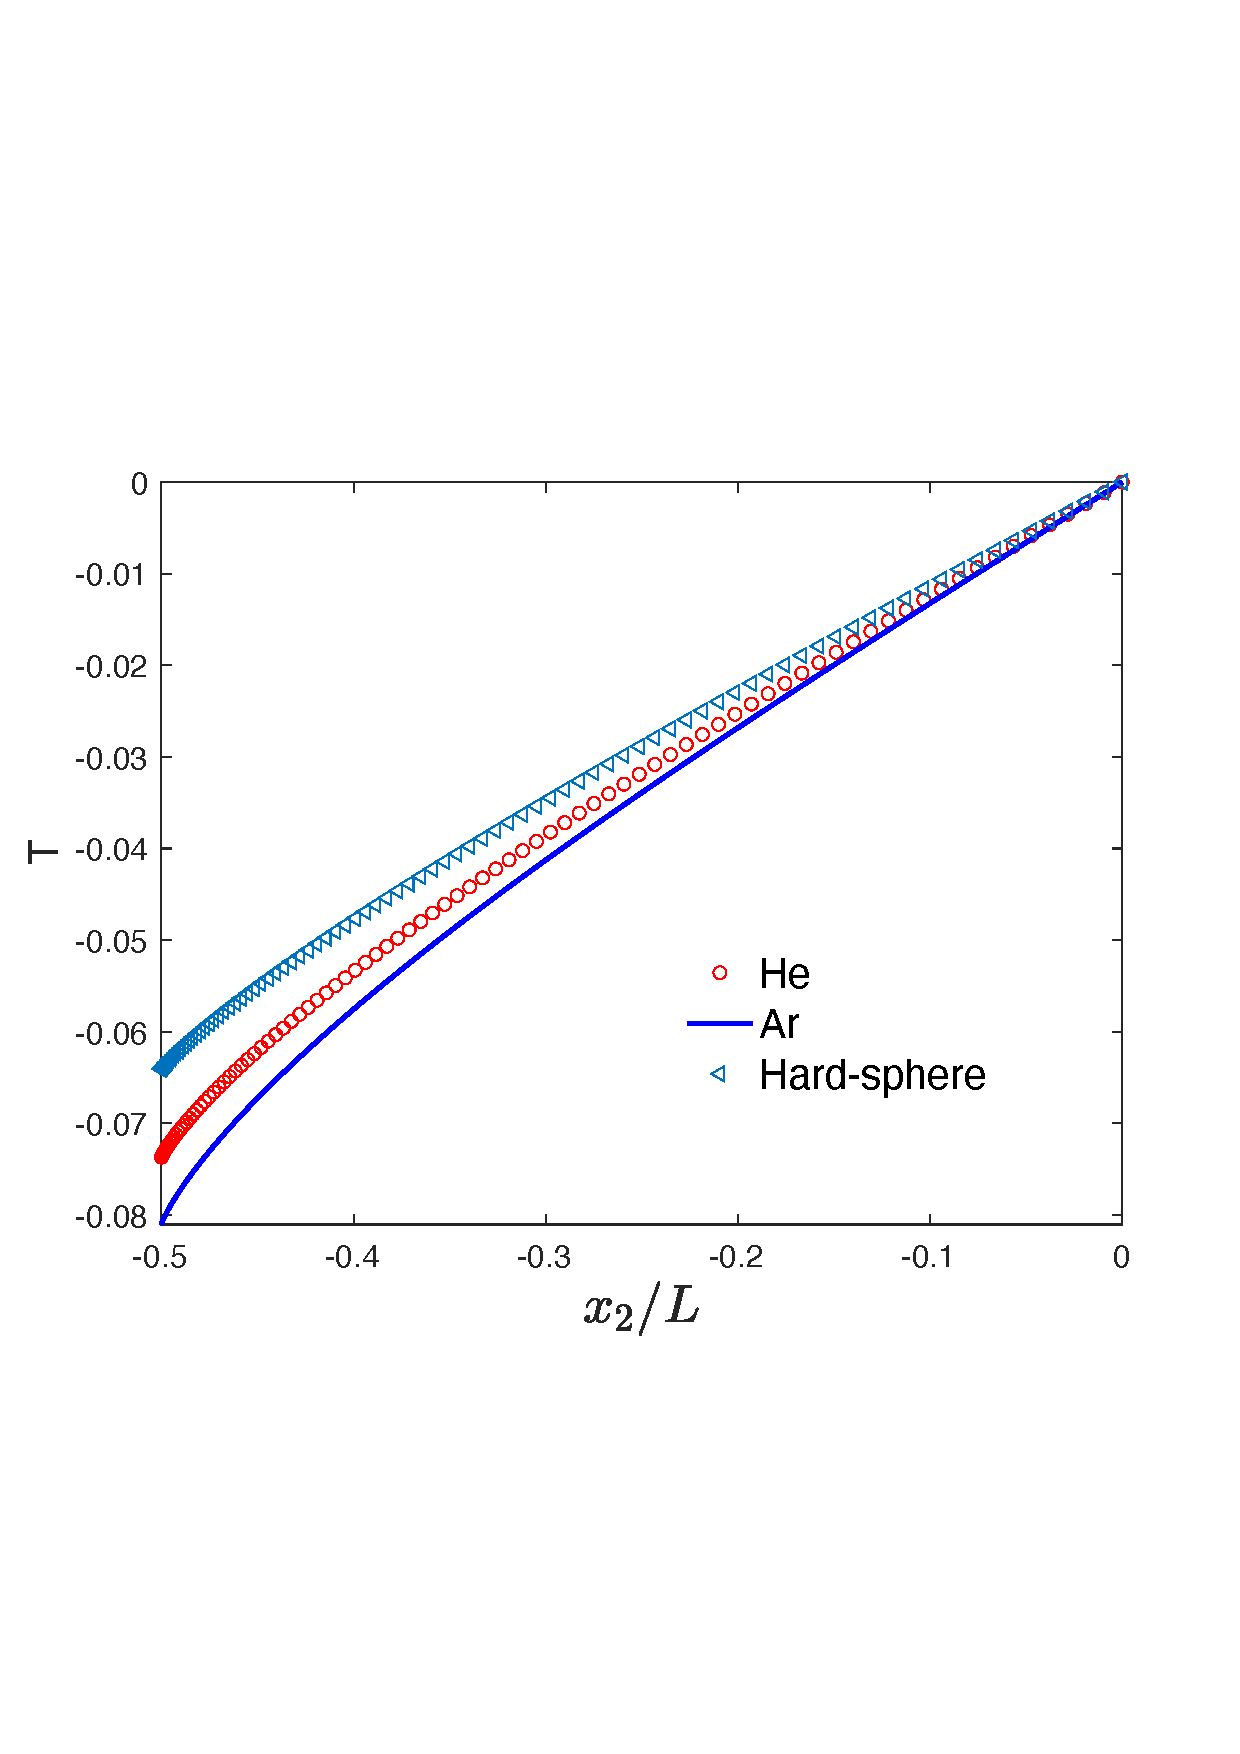
\includegraphics[scale=0.35]{FourierDelta01T}\\
	\vskip 0.5cm
	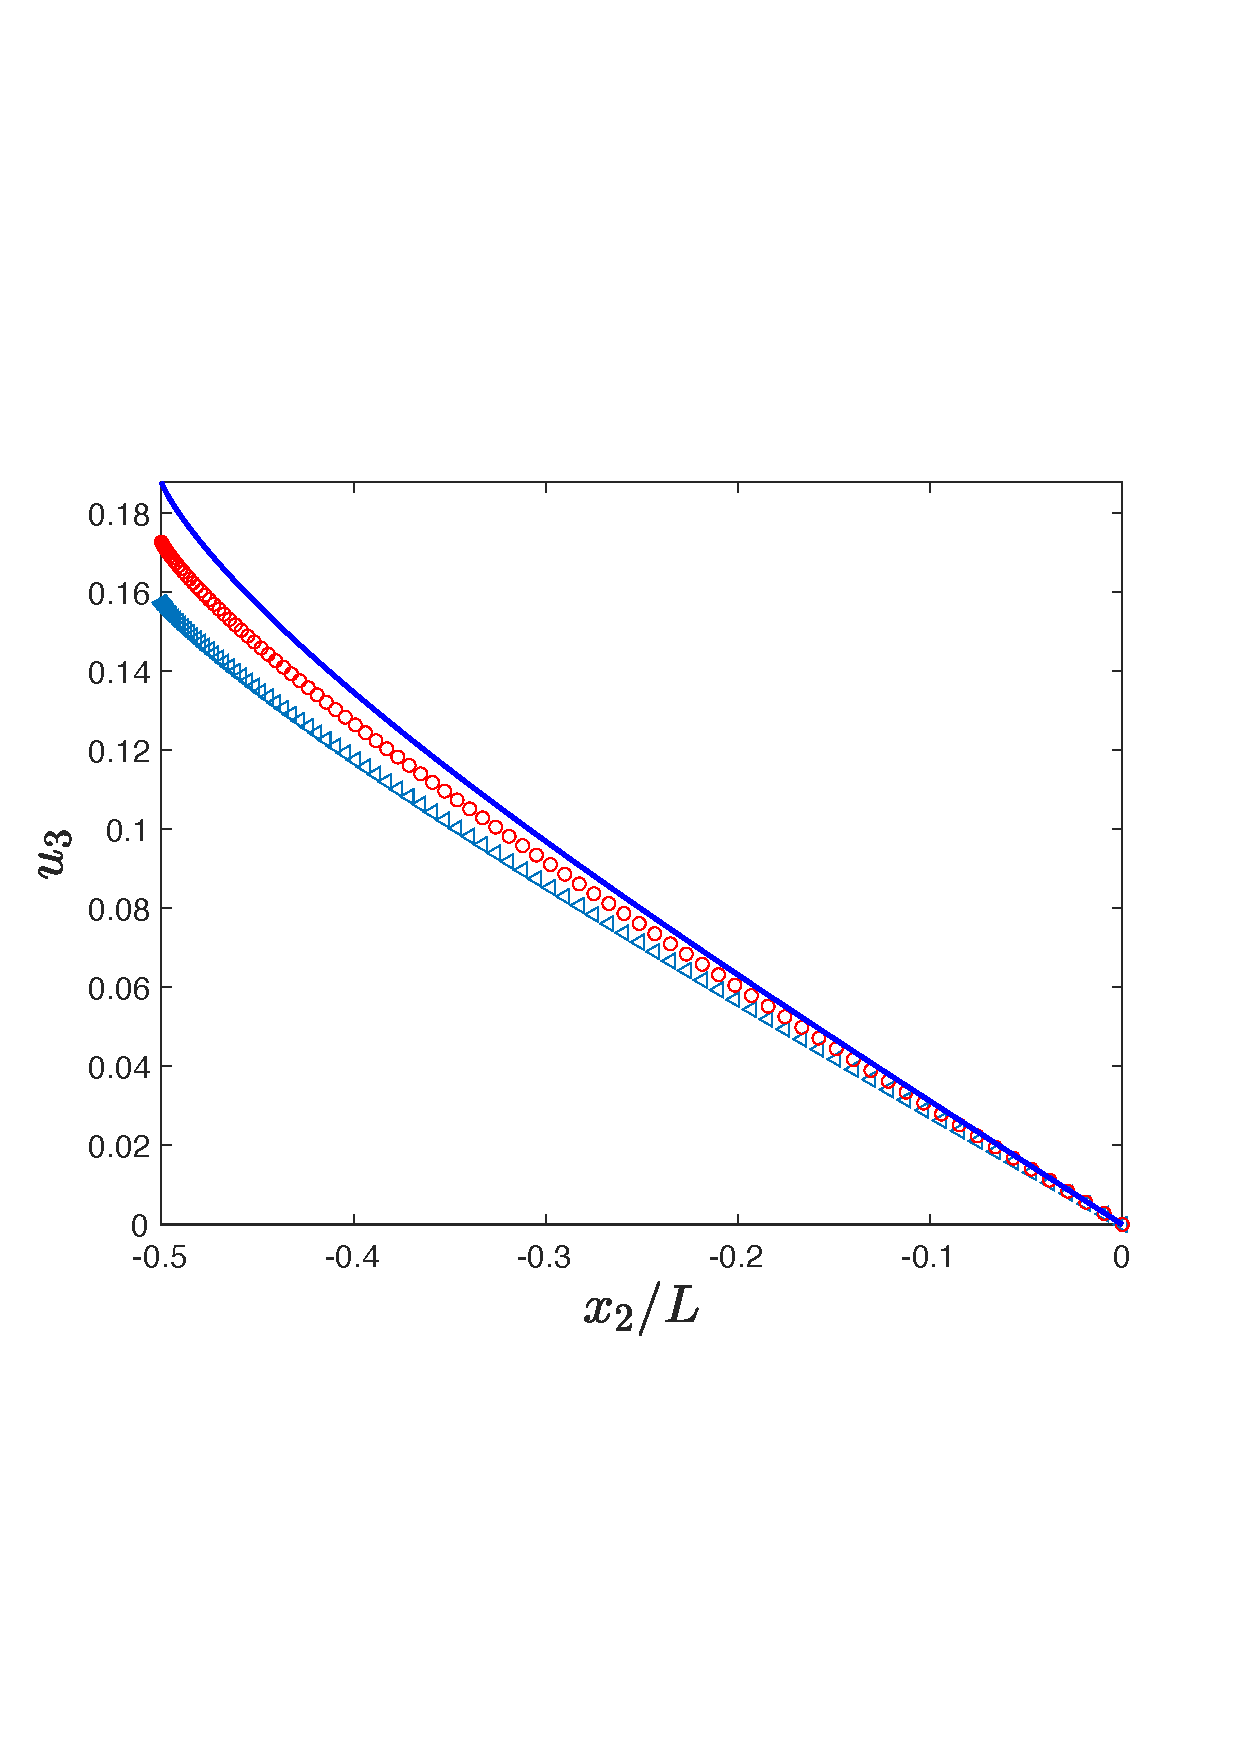
\includegraphics[scale=0.35]{LJCouetteDelta01V}
	\caption{
		(Top) Normalized density and temperature profiles in the linearized Fourier flow of various gases between two parallel plates. (Bottom) Velocity profiles in the linearized planar Couette flow. The rarefaction parameter is $\delta_{rp}=0.1$. 
	}
	\label{Fourier_lin}
\end{figure}

The geometry is the same as that of the Poiseuille flow, except that the plate at $x_2=-1/2$ has a temperature $T_0-\Delta{T}/2$, while the plate at $x_2=1/2$ has a temperature $T_0+\Delta{T}/2$. Also, there is no pressure gradient along the $x_1$ and $x_3$ directions. The temperature difference $\Delta{T}$ is negligible compared to $T_0$, so that the Boltzmann equation~\eqref{Boltzmann_dimensionless} can be linearized to Eq.~\eqref{Chapter1_Boltzmann_lin} by choosing as $\beta=\Delta{T}/T_0$. Assuming diffuse gas-wall interaction, the BC at $x_2=-\frac{1}{2}$ with ${v_2>0}$ reads
\begin{equation}
h= \left[ 1-\frac{1}{2}v^2-2\sqrt{\pi}\int_{v_2<0} v_2h\left(v,x_2=-\frac{1}{2}\right)dv\right] f_{eq}, 
\end{equation}
while at $x_2=0$, symmetry leads to $h(v_1,v_2,v_3)=-h(v_1,-v_2,v_3)$ when $v_2<0$.

%The spatial region $-1/2\le{x_2}\le0$ is discretized by 100 non-uniform grid points, with most of the grid points located near the wall, see Eq.~\eqref{spatial_d}. The three-dimensional molecular velocity domain $[-6,6]^3$ is discretized by $32\times128\times32$ grid points, and the number of frequency components is $32\times48\times32$.  

%The iterative scheme ${v_2}{\partial h^{(k+1)}}/{\partial x_2}+\nu_{eq}(v)h^{(k+1)}=\mathcal{L}^+(h^{(k)})$ is used, and the iterations are terminated when the maximum relative difference in the density $n=\int hdv$, temperature $T=2\int hv^2dv/3-n$, and heat flux $q_2=\int hv^2v_2dv$ between two consecutive steps is less than $10^{-5}$. 


Typical density and temperature profiles are shown in Fig.~\ref{Fourier_lin} for a rarefaction parameter of $\delta_{rp}=0.1$ and $T_0=300$~K. Although they have the same shear viscosity, the macroscopic properties of the six gases are quite different.  At the wall, when $\delta_{rp}=0.1$, the relative difference in  density between He and the HS gas is 22\%. This difference between LJ and HS potentials increases as $k_BT_0/\epsilon$ decreases: the density of Xe at the wall is 40\% larger than that of the HS gas. For the temperature, the largest difference between the noble gases and the HS gas reaches 25\%. As $\delta_{rp}$ increases, relative differences in the densities and the temperature decreases: when $\delta_{rp}=1$, relative differences in the density and temperature of the HS gas and Xe at the wall are reduced to 11.4\% and 8.7\%, respectively, while they are 1.8\% and 1.5\% by $\delta_{rp}=10$. As $\delta_{rp}$  further increases, the hydrodynamic flow regime is reached and there is no difference between various gases. Interestingly, the differences in heat flux between various gases is small.



%
%\subsection{Couette flow}
%\index{Couette flow}
%The geometry is the same as that in the Poiseuille flow, except that the plate at $x_2=-\ell/2$ moves in the $x_3$ direction with a speed $u_{w}$, while the other plate moves in the opposite direction with the same speed. Also, there is no pressure gradient along the $x_1$ and $x_3$ directions. When the wall speed is far less than the most probable speed $v_m$, the Boltzmann equation is linearized to Eq.~\eqref{Chapter1_Boltzmann_lin} by choosing $\beta=u_{w}/v_m$. The diffuse gas-wall BC becomes $h(v,x_2=-0.5)=2v_3f_{eq}$ for $v_2>0$, and $h(v_1,v_2,v_3,x_2=0)=h(v_1,-v_2,-v_3,x_2=0)$ for $v_2<0$ due to symmetry. 
%
%%We are interested in the gas velocity and shear stress. The velocity, which is normalized by the wall speed, is $u_3=\int hv_3dv$; the shear stress, which is normalized by $n_0k_BT_0u_{wall}/v_m$, is $p_{23}=2 \int hv_2v_3dv$.
%
%
%Figure~\ref{Fourier_lin} depicts the typical velocity profiles when $\delta_{rp}=0.1$, where the influence of the molecular potential is clearly seen.  As $\delta_{rp}$ increases, the difference in the velocity profiles of the six gases decreases. For instance, the relative difference between the HS gas and Xe decreases from 22.3\% when $\delta_{rp}=0.1$, to 4.5\% at $\delta_{rp}=1$, and to 0.5\% by $\delta_{rp}=10$. Similar to heat fluxes in the Fourier flows, the relative differences in shear stress between the various gases in Couette flow is small, and first increases and then decreases with $\delta_{rp}$ .

%
%\leir{effect shear viscosity and thermal conductivity}
%\newpage


\section{Cercignani-Lampis boundary condition}
\index{Cercignani-Lampis boundary condition}
% data used in Chapter 2: kinetic boundary conditions

We present solutions of the LBE for the Poiseuille flow between two infinite parallel plates and through a circular cross section. Although this classical problem has been investigated extensively, accurate numerical results based on the LBE and the Cercignani-Lampis  BC is scarce. 

%With the state-of-the-art numerical method, the mass and heat flow rates of the Poiseuille flow and thermal transpiration are obtained with the Cercignani-Lampis BC, which provides critical data to assess the gas kinetic boundary conditions in Chapter~\ref{chap:BoundaryCondition}.


\begin{figure}[t]
	\centering
	{	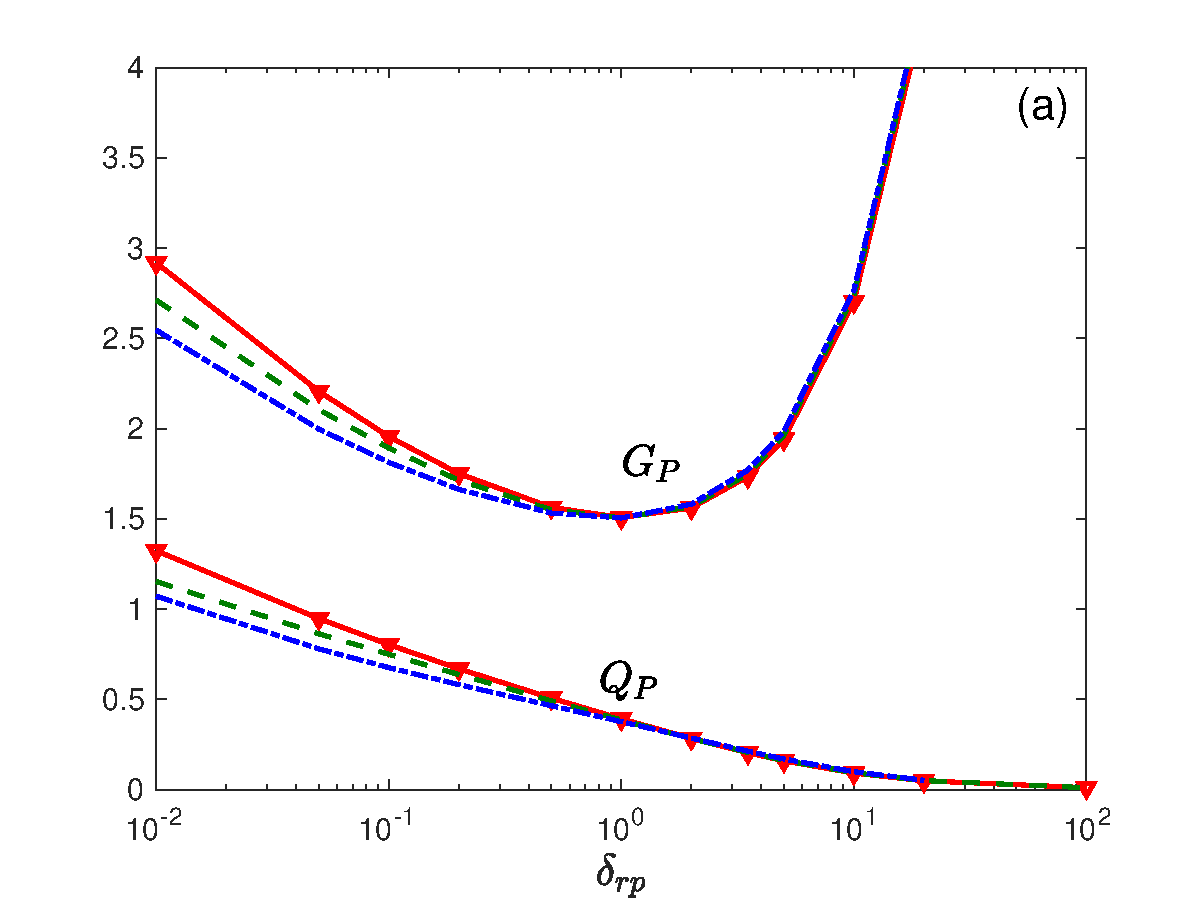
\includegraphics[scale=0.35]{BC_Fig2a.eps}}
	{	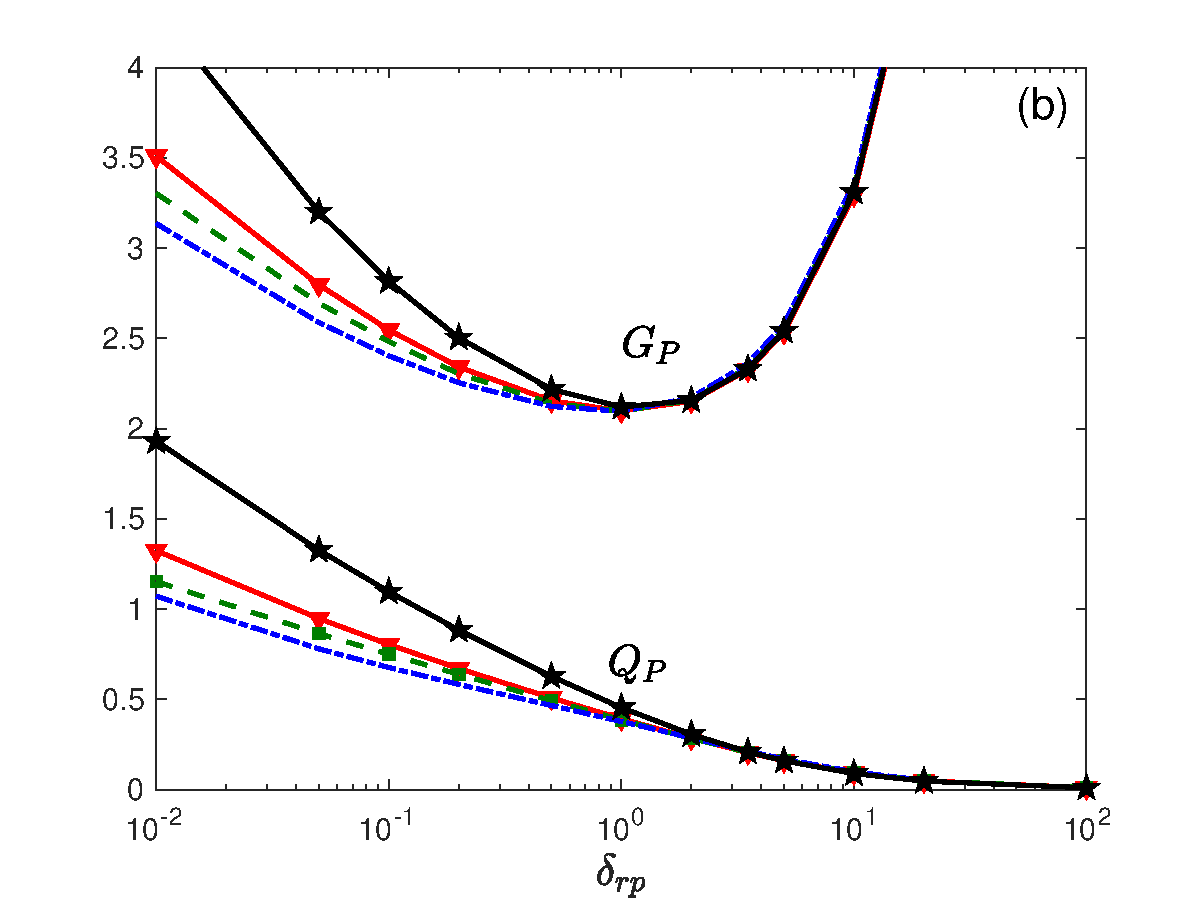
\includegraphics[scale=0.35]{BC_Fig2b.eps}}\\
	\vskip 0.3cm
	{	\includegraphics[scale=0.35]{BC_Fig2c.eps}}
	\caption{
		The MFR and HFR in the Poiseuille flow between two parallel plates, when the Cercignani-Lampis and Maxwell BCs are used. Triangles: HS molecules. Dashed lines: Helium. Dash-dotted lines: Xenon. When the Lennard-Jones potentials is used, the wall temperature is $T_w=300$~K. In the Cercignani-Lampis   BC, we use $\alpha_n=1$,  (a) $\alpha_t=1$ and (b) $\alpha_t=0.75$. In the Maxwell   BC, $\alpha_M=0.75$ is used (Pentagrams). (c) The TPD exponent. 
	} 
	\label{Chapter_BC_Pois1D}
\end{figure}


For the Cercignani-Lampis  BC, the scattering kernel~\eqref{CL} is simplified
to~\citep{Sharipov2002CL,Sharipov2003CL,SharipovCL3}: 
\begin{equation}
R_{CL}(\bm{v}^{\prime}\rightarrow \bm{v})=R_n(v_n^{\prime}\rightarrow%
{v_n})R_t(\bm{v}_t^{\prime}\rightarrow{\bm{v}_t}),
\end{equation}
where 
\begin{equation*}  
\begin{aligned}[b] R_n(v_n'\rightarrow{v_n})=&\frac{2v_n}{\alpha_n}
I_0\left(2\frac{\sqrt{1-\alpha_n}v_nv_n'}{\alpha_n}\right)\exp\left\{-%
\frac{[v_n^2+(1-\alpha_n)v_n']^2}{\alpha_n} \right\},\\
R_t(\bm{v}_t'\rightarrow{\bm{v}_t})=&\frac{1}{\pi\alpha_t(2-%
	\alpha_t)}\exp\left[-\frac{|\bm{v}_t-(1-\alpha_t)\bm{v}_t'|^2}{%
	\alpha_t(2-\alpha_t)} \right]. 
\end{aligned}
\end{equation*}

\subsection{Flow through parallel plates}

We first consider the Poiseuille flow between two infinite parallel plates at a distance $L $. Table~\ref{table_poiseuille_1d_BC} shows the MFR and HFR for HS molecules, when the Cercignani-Lampis and Maxwell  BCs are used. When the parameters $\alpha _{n}$, $\alpha _{t}$, and $\alpha _{M}$ in the Cercignani-Lampis and Maxwell  BCs are fixed, the HFR always increases when the rarefaction parameter $\delta_{rp} $ decreases, while the MFR first decreases and then increases with $\delta_{rp} $, such that the famous Knudsen minimum is observed at $\delta_{rp} \approx 1$. 


For the Maxwell BC, when $\delta_{rp} $ is fixed, both the MFR and HFR increases significantly when the  accommodation coefficient $\alpha _{M}$ is reduced. For the Cercignani-Lampis  BC, when the values of $\delta_{rp} $ and $\alpha _{n}$ are fixed, the MFR also increases rapidly when $\alpha _{t}$ decreases. From Eq.~\eqref{chi_CL} we know that $\alpha _{t}$ is the effective TMAC of the Cercignani-Lampis  BC. By choosing $\alpha _{M}=\alpha _{t}$, we see in Table~\ref{table_poiseuille_1d_BC} that the MFR from the Cercignani-Lampis  BC increases slower than that of the Maxwell  BC, as $\alpha _{t}$ and $\alpha_{M}$ decrease.





From the numerical simulation we see that the influence of $\alpha _{n}$ on MFR is  very limited. When $\alpha _{t}$ and $\delta_{rp}$ are fixed, the MFR decreases slightly when $\alpha _{n}$ increases. For instance, for $\delta_{rp} =0.01$, the MFR is decreased by 10\% when $\alpha _{n}$ is increased from 0.25 to 1; as $\delta_{rp} $ increases, this influence becomes weaker and weaker. 


	

\begin{table}[t]
	\centering
	\caption{Dimensionless flow rates in the Poiseuille flow of HS molecules
		between two infinite parallel plates, obtained from the LBE with the
		Cercignani-Lampis  BC. }
	\begin{tabular}{clccclccccccc}
		\hline
		&  & ${G}_P$ & ${Q}_P$ & ${G}_P$ & ${Q}_P$ & ${G}_P$ & ${Q}_P$ & ${G}_P$
		& ${Q}_P$  \\ 
		$\delta_{rp}$ & $\alpha_t$ & \multicolumn{2}{c}{$\alpha_n$=0.25} & 
		\multicolumn{2}{c}{$\alpha_n$=0.5} & \multicolumn{2}{c}{$\alpha_n$=0.75} & 
		\multicolumn{2}{c}{$\alpha_n$=1} & 
		\\ 
		\hline
		0.01 & 0.5 & 5.115 & 1.699 & 4.871 & 1.499 & 4.752 & 1.390 & 4.684 & 1.322 &  \\ 
		& 1 & 2.911 & 1.320 & 2.911 & 1.320 & 2.911 & 1.320 & 2.911 & 1.320 &   \\ 
		& 1.5 & 2.084 & 1.122 & 2.196 & 1.205 & 2.265 & 1.265 & 2.320 & 1.319 &   \\ 
		0.1 & 0.5 & 3.996 & 1.098 & 3.854 & 0.953 & 3.774 & 0.866 & 3.724 & 0.807 & 
		\\ 
		& 1 & 1.951 & 0.801 & 1.951 & 0.801 & 1.951 & 0.801 & 1.951 & 0.801 &  \\ 
		& 1.5 & 1.200 & 0.634 & 1.270 & 0.699 & 1.319 & 0.749 & 1.360 & 0.796 &   \\ 
		0.2 & 0.5 & 3.710 & 0.906 & 3.616 & 0.798 & 3.558 & 0.726 & 3.519 & 0.675 &   \\ 
		& 1 & 1.747 & 0.667 & 1.747 & 0.667 & 1.747 & 0.667 & 1.747 & 0.667 &   \\ 
		& 1.5 & 1.037 & 0.525 & 1.086 & 0.577 & 1.123 & 0.620 & 1.156 & 0.661 &    \\ 
		1 & 0.5 & 3.308 & 0.458 & 3.297 & 0.435 & 3.288 & 0.415 & 3.280 & 0.398 &   \\ 
		& 1 & 1.507 & 0.389 & 1.507 & 0.389 & 1.507 & 0.389 & 1.507 & 0.389 &   \\ 
		& 1.5 & 0.894 & 0.336 & 0.901 & 0.351 & 0.908 & 0.366 & 0.915 & 0.381 &   \\ 
		2 & 0.5 & 3.340 & 0.300 & 3.339 & 0.296 & 3.338 & 0.292 & 3.337 & 0.288 &   \\ 
		& 1 & 1.564 & 0.281 & 1.564 & 0.281 & 1.564 & 0.281 & 1.564 & 0.281 &  \\ 
		& 1.5 & 0.970 & 0.265 & 0.971 & 0.268 & 0.971 & 0.272 & 0.972 & 0.275 &  \\ 
%		3.5 & 0.5 & 3.518 & 0.201 & 3.517 & 0.203 & 3.516 & 0.204 & 3.515 & 0.206 &  \\ 
%		& 1 & 1.742 & 0.202 & 1.742 & 0.202 & 1.742 & 0.202 & 1.742 & 0.202 &  \\ 
%		& 1.5 & 1.148 & 0.203 & 1.149 & 0.202 & 1.150 & 0.200 & 1.150 & 0.198 & \\ 
		10 & 0.5 & 4.522 & .0834 & 4.514 & .0861 & 4.508 & .0887 & 4.503 & .0912 &   \\ 
		& 1 & 2.729 & .0900 & 2.729 & .0900 & 2.729 & .0900 & 2.729 & .0900 & \\ 
		& 1.5 & 2.120 & .0962 & 2.127 & .0938 & 2.133 & .0913 & 2.138 & .0889 &  \\ 
		20 & 0.5 & 6.162 & .0437 & 6.151 & .0454 & 6.142 & .0470 & 6.133 & .0485 &  \\ 
		& 1 & 4.360 & .0480 & 4.360 & .0480 & 4.360 & .0480 & 4.360 & .0480 &  \\ 
		& 1.5 & 3.743 & .0519 & 3.752 & .0505 & 3.761 & .0490 & 3.769 & .0474&  \\ 
%		100 & 0.5 & 19.47 & .0091 & 19.45 & .0094 & 19.44 & .0098 & 19.43 & .0102 &  \\ 
%		& 1 & 17.66 & .0101 & 17.66 & .0101 & 17.66 & .0101 & 17.66 & .0101 &  \\ 
%		& 1.5 & 17.03 & .0110 & 17.05 & .0107 & 17.06 & .0103 & 17.07 & .0100 &  \\
		\hline
	\end{tabular}%
	\label{table_poiseuille_1d_BC}
\end{table}




The variation of HFR with respect to $\alpha _{n}$ and $\alpha _{t}$ is more complicated than that of the MFR. First, when $\alpha _{n}$ and $\delta_{rp}$ are fixed, the HFR increases slightly with $\alpha _{t}$ at large values of $\delta_{rp} $, while it increases with decreasing $\alpha _{t}$ at small values of $\delta_{rp} $. Second, when $\alpha _{t}=1$ and $\delta_{rp} $ is fixed, the HFR does not change with $\alpha _{n}$: in fact, in this case it can be proven that the Cercignani-Lampis  BC is reduced to the diffuse  BC~\citep{Sharipov2002CL}. Third, when $\alpha_{t}(\neq1)$ and $\delta_{rp} $ are fixed, the HFR increases slightly with $\alpha _{n}$ at large values of $\delta_{rp}$, but it increases with decreasing $\alpha _{n}$ at smaller values of $\delta_{rp} $. Similar behaviors have been observed by~\cite{Sharipov2002CL} when the linearized Shakhov kinetic model is used instead of the LBE.

The influence of intermolecular potential is also investigated. For this we choose helium and xenon, since from~\cite{Sharipov2009} it is known that the results of other noble gases such as neon, argon, and krypton will lie between helium and xenon. Some typical MFR and HFR profiles are shown in Fig.~\ref{Chapter_BC_Pois1D}, from which we see that the influence of intermolecular potential is obvious at small values of $\delta_{rp}$, irrespective of the gas-surface  BCs. For small values of $\delta_{rp}$ (i.e. $\delta_{rp} <1$), among the HS gas, helium, and xenon, the HS gas has the largest MFR and HFR, while xenon has the smallest: in the diffuse  BC, the relative differences in the MFR and HFR between HS gas and xenon are about 15\% when $\delta_{rp} =0.01$. In the Cercignani-Lampis  BC with $\alpha _{n}=1$ and $\alpha _{t}=0.75$, the relative differences in the MFR and HFR between HS gas and xenon are about 12\% and 23\%, respectively, when $\delta_{rp} =0.01$.


Figure~\ref{Chapter_BC_Pois1D}(c) also shows the exponent of thermal pressure difference (TPD), which is an important parameter determining the performance of a Knudsen pump. 
In the range of $\delta_{rp} $ considered, the HS gas has the largest TPD, while xenon has the smallest. This difference increases when $\delta_{rp} $ decreases. For instance, in the diffuse  BC, the relative difference in TPD exponent between the HS gas and xenon is about 8\% when $\delta_{rp} =0.01$. In the Cercignani-Lampis  BC, when $\delta_{rp}$ is fixed, the TPD exponent decreases with $\alpha _{t}$. In the Maxwell  BC, when $\alpha _{M}$ decreases, the TPD exponent decreases at large values of $\delta_{rp} $, but at small values of $\delta_{rp} $ (free-molecular flow regime), the  accommodation coefficient $\alpha _{M}$ does not have any influence on the TPD exponent.


%	However, for the LBE, the velocity space cannot be represented in polar coordinates, since the molecular velocity along the flow direction cannot be integrated due to the nonlinear structure of the Boltzmann equation. Therefore, the LBE will be solved in polar coordinates for spatial variables, while the three-dimensional molecular velocity space is represented by cylindrical coordinates.





%
%
%\begin{figure}[t]
%	\centering 
%	\includegraphics[scale=0.4]{BC_Fig3}
%	\caption{
%		The relative error $({G}_{\text{Lennard-Jones}}/{G}_{\text{HS}}-1)\times100$ in the MFR between the Lennard-Jones and HS potentials, in the Poiseuille (dashed lines) and thermal transpiration (solid lines) flows through a tube, when the diffuse  BC is used. 
%	}
%	\label{Thermaltube}
%\end{figure}




\begin{table}[t]
	\centering
	\caption{Dimensionless flow rates in the Poiseuille flow of HS molecules through a circular tube, using the Cercignani-Lampis  BC.  The characteristic length $L$ is the radius of circular cross section.}
	\begin{tabular}{clccclccccccc}
		\hline
		&  & ${G}_P$ & ${Q}_P$ & ${G}_P$ & ${Q}_P$ & ${G}_P$ & ${Q}_P$ & ${G}_P$
		& ${Q}_P$ &  &  &  \\ 
		$\delta_{rp}$ & $\alpha_t$ & \multicolumn{2}{c}{$\alpha_n$=0.25} & 
		\multicolumn{2}{c}{$\alpha_n$=0.5} & \multicolumn{2}{c}{$\alpha_n$=0.75} & 
		\multicolumn{2}{c}{$\alpha_n$=1} &  &  &  \\
		\hline 
		0 & 0.5 & 3.401 & 1.026 & 3.356 & 0.912 & 3.328 & 0.838 & 3.309 & 0.786 &  & 
		&  \\ 
		& 1 & 1.504 & 0.752 & 1.504 & 0.752 & 1.504 & 0.752 & 1.504 & 0.752 &  &  & 
		\\ 
		& 1.5 & 0.838 & 0.608 & 0.856 & 0.646 & 0.871 & 0.684 & 0.887 & 0.725 &  & 
		&  \\ 
		0.01 & 0.5 & 3.363 & 0.989 & 3.321 & 0.881 & 3.295 & 0.809 & 3.277 & 0.759 & 
		&  &  \\ 
		& 1 & 1.472 & 0.725 & 1.472 & 0.725 & 1.472 & 0.725 & 1.472 & 0.725 &  &  & 
		\\ 
		& 1.5 & 0.809 & 0.584 & 0.825 & 0.620 & 0.840 & 0.657 & 0.855 & 0.697 &  & 
		&  \\ 
		0.1 & 0.5 & 3.251 & 0.837 & 3.227 & 0.763 & 3.210 & 0.709 & 3.198 & 0.669 & 
		&  &  \\ 
		& 1 & 1.397 & 0.634 & 1.397 & 0.634 & 1.397 & 0.634 & 1.397 & 0.634 &  &  & 
		\\ 
		& 1.5 & 0.753 & 0.516 & 0.763 & 0.545 & 0.773 & 0.574 & 0.784 & 0.607 &  & 
		&  \\ 
		0.5 & 0.5 & 3.181 & 0.574 & 3.176 & 0.553 & 3.172 & 0.536 & 3.169 & 0.520 & 
		&  &  \\ 
		& 1 & 1.381 & 0.492 & 1.381 & 0.492 & 1.381 & 0.492 & 1.381 & 0.492 &  &  & 
		\\ 
		& 1.5 & 0.767 & 0.432 & 0.770 & 0.443 & 0.772 & 0.455 & 0.775 & 0.468 &  & 
		&  \\ 
		1 & 0.5 & 3.233 & 0.432 & 3.232 & 0.429 & 3.231 & 0.426 & 3.230 & 0.423 &  & 
		&  \\ 
		& 1 & 1.448 & 0.403 & 1.448 & 0.403 & 1.448 & 0.403 & 1.448 & 0.403 &  &  & 
		\\ 
		& 1.5 & 0.845 & 0.379 & 0.847 & 0.380 & 0.847 & 0.383 & 0.848 & 0.385 &  & 
		&  \\ 
		2 & 0.5 & 3.423 & 0.295 & 3.420 & 0.300 & 3.418 & 0.305 & 3.417 & 0.309 &  & 
		&  \\ 
		& 1 & 1.639 & 0.298 & 1.639 & 0.298 & 1.639 & 0.298 & 1.639 & 0.298 &  &  & 
		\\ 
		& 1.5 & 1.038 & 0.301 & 1.040 & 0.297 & 1.042 & 0.293 & 1.043 & 0.288 &  & 
		&  \\ 
		5 & 0.5 & 4.113 & 0.152 & 4.105 & 0.157 & 4.098 & 0.162 & 4.093 & 0.167 &  & 
		&  \\ 
		& 1 & 2.319 & 0.164 & 2.319 & 0.164 & 2.319 & 0.164 & 2.319 & 0.164 &  &  & 
		\\ 
		& 1.5 & 1.708 & 0.175 & 1.715 & 0.170 & 1.721 & 0.165 & 1.726 & 0.161 &  & 
		&  \\ 
		10 & 0.5 & 5.333 & .0835 & 5.322 & .0868 & 5.313 & .0899 & 5.305 & .0929 & 
		&  &  \\ 
		& 1 & 3.531 & .0917 & 3.531 & .0917 & 3.531 & .0917 & 3.531 & .0917 &  &  & 
		\\ 
		& 1.5 & 2.913 & .0992 & 2.923 & .0963 & 2.932 & .0934 & 2.939 & .0904 &  & 
		&  \\ 
		20 & 0.5 & 7.815 & .0437 & 7.802 & .0456 & 7.791 & .0472 & 7.782 & .0489 & 
		&  &  \\ 
		& 1 & 6.007 & .0484 & 6.007 & .0484 & 6.007 & .0484 & 6.007 & .0484 &  &  & 
		\\ 
		& 1.5 & 5.385 & .0527 & 5.396 & .0511 & 5.406 & .0495 & 5.416 & .0479 &  & 
		&  \\ 
		50 & 0.5 & 15.30 & .0179 & 15.28 & .0187 & 15.27 & .0194 & 15.26 & .0201 & 
		&  &  \\ 
		& 1 & 13.49 & .0200 & 13.49 & .0200 & 13.49 & .0200 & 13.49 & .0200 &  &  & 
		\\ 
		& 1.5 & 12.86 & .0218 & 12.87 & .0212 & 12.89 & .0205 & 12.89 & .0198 &  & 
		&  \\ 
		100 & 0.5 & 27.78 & .0090 & 27.77 & .0094 & 27.75 & .0098 & 27.74 & .0101 & 
		&  &  \\ 
		& 1 & 25.97 & .0101 & 25.97 & .0101 & 25.97 & .0101 & 25.97 & .0101 &  &  & 
		\\ 
		& 1.5 & 25.34 & .0110 & 25.35 & .0107 & 25.37 & .0103 & 25.38 & .0100 &  & 
		& \\
		\hline
	\end{tabular}%
	\label{table_poiseuille_tube_compare}
\end{table}

%Fig.~\ref{Thermaltube} shows the influence of  intermolecular potential on the MFR in thermal transpiration. For $\delta_{rp} >0.5$, the HS model underpredicts the MFR of the Lennard-Jones potentials, say, when $\delta_{rp} =10$, by about 8\% and 4\% for argon and helium, respectively. When $\delta_{rp} <0.5$, however, the HS model overpredicts the MFR. When $\delta_{rp} \rightarrow 0$, the intermolecular potential has no influence on the dimensionless mass flow rate. On the other hand, the influence of intermolecular potential in the MFR of  Poiseuille flow is within 2\% for all the rarefaction parameters considered.


\subsection{Flow through long tube}

For flows through circular cross sections, the  polar coordinates can be applied to reduce the computational cost significantly. Introducing the transformation $x_1=r\cos\theta$, $x_2=r\sin\theta$, $v_1=v_r\cos\theta$,  $v_2=v_r\sin\theta$, and defining the VDF $h=h(r,\theta,v_r,v_3)$ in cylindrical (molecular velocity)-polar (space) coordinates $v_r\in[0,+\infty)$, $\theta\in[0,2\pi]$, $v_z\in(-\infty,\infty)$, and $r\in[0,1]$, the LBE can be written as:
\begin{equation}\label{polar}
v_1\frac{\partial h}{\partial r}-\frac{v_2}{r}\frac{\partial h}{\partial \theta}=\mathcal{L}^+(h)-\nu_{eq}{h} -v_3f_{eq}. 
\end{equation}

In the numerical simulation, the spatial coordinate $r$ is discretized into 150 nonuniform points, with most of the points located near the pipe surface $r=1$. Due to symmetry, the truncated velocity $v_r\in(0,4)$ is discretized into 64 nonuniform points, with most of the points located near $v_r=0$, while $\theta\in[0,\pi]$ and $v_3\in(0,6)$ are discretized into 40 and 12 uniform points, respectively. The linearized Boltzmann collision operator is approximated by FSM in the following way: first, the spectrum of the VDF is calculated by Fourier transform from the cylindrical molecular velocity space to the Cartesian frequency space. Second, the FSM is applied to find the spectrum of the linearized Boltzmann collision operator in the Cartesian coordinate. Finally, the inverse Fourier transform is used to find the collision operator in the cylindrical space. 

% Unlike the Poiseuille flow between two parallel plates, where the MFR and HFR increase logarithmically as $-\ln\delta_{rp}$ when $\delta_{rp} \rightarrow 0$~\citep{Takata2011}, both approach constant values when $\delta_{rp} \rightarrow 0$. 

The flow rates of the Poiseuille flow through a long tube are shown in Table~\ref{table_poiseuille_tube_compare}. The influence of BC on the dimensionless flow rates is similar to that between two parallel plates. 
